\documentclass[a4paper, twoside, openany, usecolor, 12pt]{CNSDANthesisEN}
% The usecolor option sets the titles in blue, as requested by
% the Ghent University housestyle. Remove this to get a black
% and white version of things.
\usepackage[english]{babel} %Use dutch headings and titles

%-------------------------------------------------------------------------------
% FILL IN YOUR DETAILS
%
% Keep in mind that UGent doesn't use copromotors any longer. However,
% if it is required to add, please uncomment the line starting with
% \copromotor below and fill in the correct details.
%
\title{Explaining graph neural networks for chemical application with structure aware games}
\author{Xander Wieme}

\studentnr{01802113} % Fill in your student number

\promotor{Prof. Dr. Yvan Saeys}
%\copromotor{Dr. FirstName LastName}
\tutor{Drs. Arne Gevaert}

\orientation{Statistical Data Analysis}

\academicyear{2023 - 2024}

%-------------------------------------------------------------------------------
% The preamble. Note that the following packages are already loaded by
% the class bwthesis: geometry, amsmath, amsfonts, amssymb, graphicx,
% xcolor, ulem, setspace

% This package provides the lstlisting environment for formatting your code.
% To set the parameters like language or layout, look at the help for the
% listings package and adapt the file listingfile.tex accordingly.
% 
\usepackage{listings}
\definecolor{mygreen}{rgb}{0,0.6,0}


\lstset{ %
	language=R,                % choose the language of the code
	basicstyle=\footnotesize\ttfamily,       % the size of the fonts that are used for the code
	numbers=left,                   % where to put the line-numbers
	numberstyle=\scriptsize,      % the size of the fonts that are used for the line-numbers
	stepnumber=1,                   % the step between two line-numbers. If it is 1 each line will be numbered
	numbersep=5pt,                  % how far the line-numbers are from the code
	backgroundcolor=\color{white},  % choose the background color. You must add \usepackage{color}
	showspaces=false,               % show spaces adding particular underscores
	showstringspaces=false,         % underline spaces within strings
	showtabs=false,                 % show tabs within strings adding particular underscores
	frame=none,           % adds a frame around the code
	tabsize=2,          % sets default tabsize to 2 spaces
	captionpos=b,           % sets the caption-position to bottom
	breaklines=true,        % sets automatic line breaking
	breakatwhitespace=false,    % sets if automatic breaks should only happen at whitespace
	xleftmargin=15pt,
	xrightmargin=5pt,
	commentstyle=\color{mygreen}, %teal
	keywordstyle=\color{blue},
	stringstyle=\color{orange}       % if you want to add LaTeX within your code
} % contains settings for the package listings
% this package provides an environment for algorithms (cfr. Pseudocode)
\usepackage[ruled]{algorithm2e} 
% This package provides extra possibilities for tables
\usepackage{booktabs}
% this package is used to produce both author-date and standard numerical citations for BibTeX btibliographies
\usepackage[super,square,numbers]{natbib}
% This packages adds the Appendix name in the toc. See below
\usepackage[titletoc]{appendix}

\usepackage{mathtools}
\usepackage{mathptmx}
\usepackage{cleveref}
\usepackage{longtable}

\newcommand*{\citen}[1]{%
  \begingroup
    \romannumeral-`\x % remove space at the beginning of \setcitestyle
    \setcitestyle{numbers}%
    \cite{#1}%
  \endgroup   
}

% ---- ADDITIONAL SETTINGS
\graphicspath{{Fig/}} % path to the figure directory
% \setcitestyle{numbers}

%-------------------------------------------------------------------------------
% The actual document
%
\begin{document}


% This file should not be changed, apart from filling in the date
% if necessary. 
% In the odd chance something goes wrong with the filling in of the names,
% you can change those at the locations indicated in the comments below.

\par\vspace*{\fill}

The author and promoter give permission to consult this master dissertation and to copy it or parts of it for personal use. Every other use falls under the restrictions of the copyright, in particular concerning the obligation to mention explicitly the source when using results of this master dissertation.

\vspace{1cm}

Gent, \today % Replace \today with the correct date if necessary !!!

\vspace{1cm}

\begin{minipage}[t][4cm][t]{0.5\textwidth}
\raggedright
The promotor,

\vspace{2.5cm}

\insertpromotor % Change if multiple names are necessary
\end{minipage}
\begin{minipage}[t][4cm][t]{0.48\textwidth}
\raggedright
The author,

\vspace{2.5cm}

\insertauthor % change if your name should be different
\end{minipage}

\thispagestyle{empty} 


\clearpage{\pagestyle{empty}\cleardoublepage}

%------------------------------------------------------------------------
\frontmatter
\pagestyle{frontmatter} %sets headers and footers correctly

% ------------ thanks -----------
\chapter{Acknowledgements}

% Here you fill in your acknowledgements
Thank you all!



% ------------ table of contents ---------
{
	\singlespacing % to keep the TOC within boundaris
	\tableofcontents
}

\addcontentsline{toc}{chapter}{Contents} %add TOC to the TOC


% ------------ summary ----------
\chapter{Abstract}

% This document should contain your abstract. 

insert english abstract here...




% The following can be commented out to remove the list of figures
% and the list of tables, as specified by the guidelines of BW
% \listoffigures
% \listoftables

%-----------------------------------------------------------------------
\mainmatter
\pagestyle{mainmatter} % sets headers and footers correctly

% Here you can add more chapters in case it is needed
\chapter{Introduction}


Prediction of molecular properties allows the filtering of molecular data sets, 
resulting in fewer wet lab experiments and a reduced development time of novel 
drugs and materials.\cite{adelusi2022molecular} However, ab initio quantum chemical algorithms are currently 
intractable due to their high computational cost.\cite{szabo2012modern} Therefore, more efficient 
algorithms are necessary, considering that the chemical space of drugable molecules 
is estimated to be $10^{60}$. One approach is machine learning (ML) algorithms, as these 
algorithms can find complicated patterns in large data sets.\cite{gorgulla2022emerging} The problem with ML 
algorithms is their black-box nature, which limits the creation of novel scientific 
knowledge and can result in trust issues in performance-critical and highly regulated 
environments.\cite{carvalho2019machine}


Explainable artificial intelligence (XAI) tries to get insight into black-box 
ML models.\cite{carvalho2019machine, yuan2022explainability} 
Current XAI methods focus on the ML model and often neglect domain 
knowledge of the studied problem. For example, when molecules are represented 
as graphs using the Lewis structure\cite{ahmad1992drawing}, common XAI techniques will search for the 
most important nodes or subgraphs to explain molecular property prediction.\cite{wu2023chemistry} The 
resulting explanation, however, is not chemically relevant as chemists are used 
to thinking in terms of substructures such as functional groups. Recently, Wu et. 
al. developed an attribution based XAI method that first partitions the molecular graph into 
chemically meaningful substructures. Therefore, their method, substructure graph 
exploration (SME), can produce chemically intuitive explanations.\cite{wu2023chemistry}


SME takes the difference between the model prediction of the molecular graph and 
the prediction of the molecular graph in which a substructure is masked. Yet, 
this approach does not consider the interaction between molecular substructures.
A commonly used attribution method in machine learning that does consider 
interactions between features is the Shapley value. Here, the Shapley value\cite{shapley1953value} will 
be used to compute the attributions of molecular graphs using a similar approach 
of Wu et. al. Since the Shapley value does not take the graphical structure of 
the input into account, the Hamiache-Navarro value\cite{hamiache_value_1999} 
is also considered to investigate whether the inclusion of the graphical structure 
can significantly improve the explanation. Comparison of the different attribution 
methods is done using pairwise Spearman rank correlation between attributions of 
different methods. The fidelity\cite{carvalho2019machine} is used to measure 
how faithful the explanation is to the model. Spearman rank correlation is also 
used to compare the ranked attributions to a manual ranks obtained using chemical 
intuition. 


The explanation methods are applied to a machine learning model that predicts the 
estimated water solubility in logS (with S the solubility in $mol/L$). Water 
solubility is chosen as the relative water solubility of a compound can be estimated 
from its molecular structure. Also, the prediction of water solubility is used 
in drugs discovery as this influences the drug blood concentration.\cite{hill2010getting}


\section{Machine learning}


Machine learning algorithms require a feature matrix $\mathbf{X} \in \mathbb{R}^{N \times p}$
where each row represents a sample and each column relates to an attribute. 
Supervised ML additionally requires a target vector $\pmb{y} \in \mathbb{R}^N$
representing another feature with a value for each sample. Then, the goal of an ML method is 
to construct a function $f$, based on parameters $\pmb{\theta}$, that can accurately 
predict the outcome variable $\pmb{y}$ of the training data $\pmb{X}$ and can 
generalize to new data.\cite{hastie2009elements} After obtaining the predicted 
values $\hat{\pmb{Y}} = f\left(\pmb{X}; \pmb{\theta}\right)$, they are compared 
to the true values $\pmb{y}$ (also called labels)
in order to determine how good the model is, which introduces the concept of loss functions $\mathcal{L}$.
Different loss functions exists for different kind of problems.\cite{wang2020comprehensive}
A commonly used loss function is the mean squared error (MSE) (\cref{eq:mse})
which averages the squared difference between the predicted value and true label.
Furthermore, optimizing the loss function with respect to the learning function
parameters produces the best model with the given architecture.\cite{hastie2009elements}


\begin{equation}
	\label{eq:mse}
	\text{MSE}\big(\pmb{y}, \pmb{X}\big) = \frac{1}{N}  \big[\pmb{y} - f(\mathbf{X})\big]^T[\pmb{y} - f(\mathbf{X})\big]
\end{equation}


One of the simplest functions $f\left(\mathbf{X}; \pmb{\theta}\right) = \mathbf{X}\pmb{\theta}$
is a linear combination of the features, where $\pmb{\theta} \in \mathbb{R}^p$
is the vector of coefficients. This model, known as linear regression, is commonly
used in statistical modeling.\cite{kutner2005applied} Although the linear model is
very interpretable, the linearity constraint is too strict which limits its
applicability. Therefore, more complicated ML algorithms were developed which are
able to obtain improved performance on complicated data with respect to linear
regression by allowing non-linear relationships.\cite{deng2012mnist} However,
they pay a price in terms of interpretability.\cite{fan2021interpretability}


\section{Neural networks}


Neural networks (NN) are a class of machine learning algorithms which are able to
approximate complicated non-linear function, inspired by the human brain.
\cite{cybenko1989approximation, rosenblatt1962principles} Although a NN is a strong
simplification of the human brain, the concept of neuron signal transit is used 
as a basic building block.\cite{wang2017origin} This signal transmission
takes place between units in a neural network. Then, different architectures
can be used to connect different units. Rosenblatt proposed a weighted sum 
of the inputs followed by a non-linear activation function.\cite{rosenblatt1962principles}
This neural network is, however, still a linear function due to its inability 
to learn non-linear functions. A solution to this limitation is stacking multiple 
perceptrons after each other, resulting in a multi layer perceptron (MLP).
The multi layer perceptron (MLP) is a basic architecture that is frequently 
utilized in other, more complicated neural networks.\cite{almeida2020multilayer}
In an MLP (\cref{fig:mlp_structure}) three parts can be distinguished: an input layer,
one or more hidden layers and an output layer.


\begin{figure}[h]
	\centering
	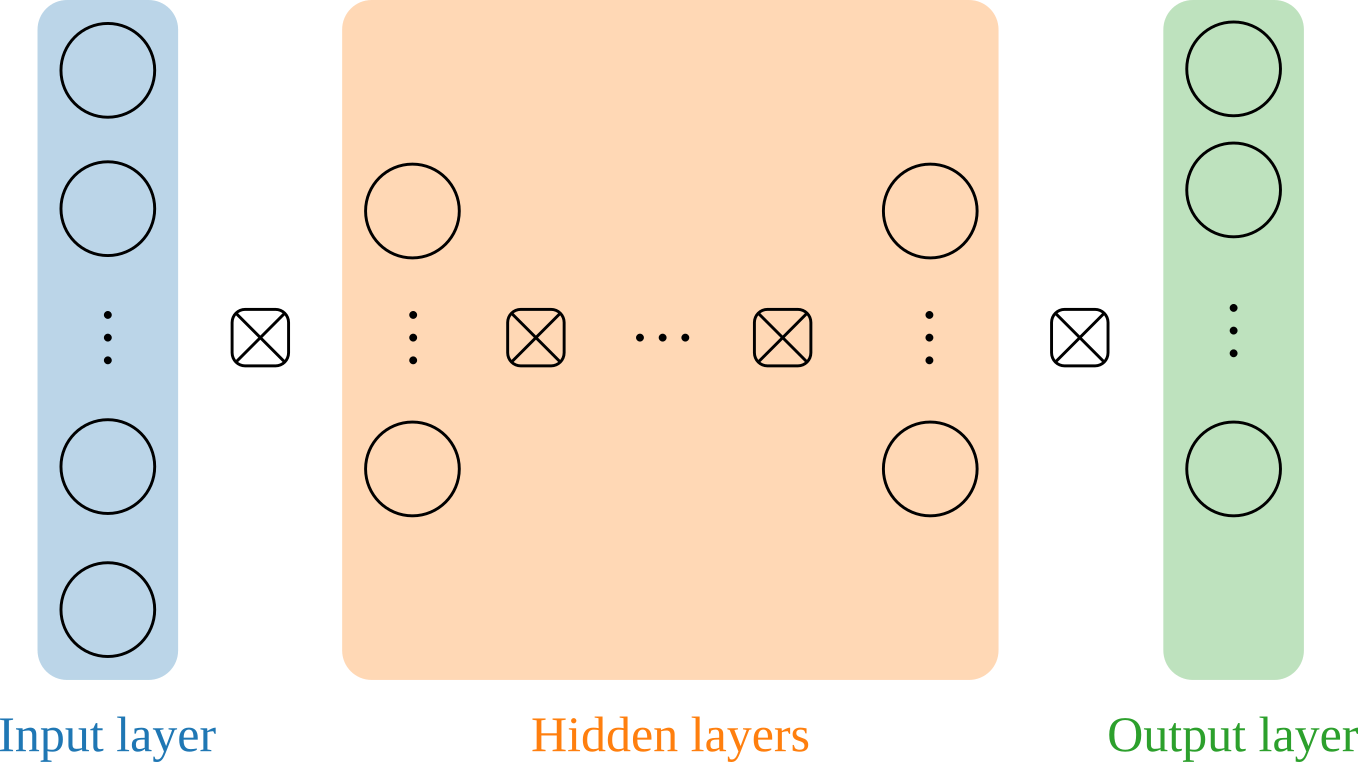
\includegraphics[scale=1.5]{mlp.png}
	\caption{General structure of a multi layer perceptron (MLP) consisting of an input layer,
		one or multiple hidden layers and an output layer. The symbol separating two layers denote that
		all neurons between these two layers are connected.}
	\label{fig:mlp_structure}
\end{figure}


The values of the input layer are equal to the given feature matrix
$\pmb{X}$. Let $n^{(1)}$ denote the number of units in the first hidden layer.
Then taking $n^{(1)}$ different linear combinations of the input layer followed by
a non-linear activation function $\sigma$ results in the values of this first hidden
layer. Generally, the values $\pmb{H}^{(l)} \in \mathbb{R}^{N \times n^{(l)}}$ of layer
$l$ are given by


\begin{equation}
	\pmb{H}^{(l)} =  \sigma^{(l)} \left(\pmb{H}^{(l-1)}\pmb{\Theta}^{(l-1)} \right),
\end{equation}


where $\pmb{\Theta}^{(l-1)} \in \mathbb{R}^{n^{(l-1)} \times n^{(l)}}$ is the weights matrix
of layer $l - 1$, with $n^{(l-1)}$ and $n^{(l)}$ the number of units in layers
$l-1$ and $l$ respectively and $\pmb{H}^{(0)} = \pmb{X}$. Popular activation
functions are listed in \cref{tab:activation_functions}.

\begin{table}[h]
	\caption{Popular activation functions used in multi layer perceptrons.}
	\label{tab:activation_functions}
	\begin{center}
		\begin{tabular}{c|c}
			\toprule
			Sigmoid(x) = $ \frac{1}{1 + e^{-x}}$                 &
			Softmax(x) = $\frac{e^x}{\sum_{i=1}^{n_L} e^{x_i}}$                                                           \\
			\midrule
			ReLU(x)\cite{glorot2011deep} = $\begin{cases}
					                                x & \text{if } x > 0 \\
					                                0 & \text{otherwise}
				                                \end{cases}$        &
			LeakyReLU(x)\cite{maas2013rectifier} =  $\begin{cases}
					                                         x        & \text{if } x > 0 \\
					                                         \alpha x & \text{otherwise}
				                                         \end{cases}$
			\\ & with $\alpha \ge 0$
			\\
			\midrule
			SeLU(x)\cite{klambauer2017self} = $\lambda \begin{cases}
					                                           x               & \text{if } x > 0 \\
					                                           \alpha(e^x - 1) & \text{otherwise}
				                                           \end{cases}$
			                                                     &
			Gelu(x)\cite{hendrycks2016gaussian} = $\begin{cases}
					                                       x            & \text{if } x > 0 \\
					                                       x \, \Phi(x) & \text{otherwise}
				                                       \end{cases}$
			\\
            see \citen{klambauer2017self} for values of $\alpha$ and $\lambda$ & with $\Phi(x)$ cumulative standard normal distribution \\
			\bottomrule
		\end{tabular}
	\end{center}
\end{table}

An MLP often does not assess the whole feature matrix at once. Rather, the feature
matrix is split up into many batches. Then, following each batch, the parameters are
updated using an optimization algorithm. Common optimization algorithms in neural networks
are gradient descent and Adam.


\subsection{Gradient descent}


A popular optimization algorithm to optimize the weights $\pmb{\Theta}$ of a neural network is
gradient descent.\cite{ruder2016overview} As the name implies, this algorithm
uses the gradient of the loss function $\mathcal{L}$ to step in the direction of the
steepest decline. The size of this step is determined by the learning rate $\alpha$.

\begin{equation}
	\pmb{\Theta}_{t+1} = \pmb{\Theta}_{t} - \alpha \nabla_{\pmb{\Theta}} \mathcal{L}
\end{equation}

Computation of the gradient can be achieved using the backpropagation algorithm, which
propagates the gradient layer by layer through the network starting at the output.
\cite{lecun1988theoretical} One limitation of gradient descent is the
fixed learning rate that has to be chosen thoughtfully at the start of training.
If the learning rate is too large, the step can pass beyond the minimum. Otherwise,
if the learning rate is too small the algorithm can take a very long time to converge.
A possible solution is to stop after a few iterations, adjust learning rate and
continue training. However, this is not really efficient. A better algorithm,
which is nowadays the standard optimization algorithm in deep learning, is Adam.\cite{kingma2014adam}


\subsection{Adam}

Adam uses exponential moving averages to estimate the first moment $m$ and 
second moment $v$ of the gradient, where the exponential decay is controlled 
by the hyperparameters $\beta_1$ and $\beta_2$. However, these moments have 
a bias towards zero due to a zero initialization. Therefore, bias correction 
is used to obtain unbiased estimates of the moments $\hat{m}$ and $\hat{v}$.\cite{kingma2014adam}


\begin{subequations}
	\begin{equation}
		m_{t+1} = \beta_1 m_t + (1 - \beta_1) \nabla_{\pmb{\Theta}} f
	\end{equation}
	\begin{equation}
		v_{t+1} = \beta_2 v_t + (1 - \beta_2) \left( \nabla_{\pmb{\Theta}} f \right)^2
	\end{equation}
	\begin{equation}
		\hat{m}_{t+1} = \frac{m_t}{1 - \beta^t_1}
	\end{equation}
	\begin{equation}
		\hat{v}_{t+1} = \frac{v_t}{1 - \beta^t_2}
	\end{equation}
\end{subequations}


Subsequently, the gradients can be updated via


\begin{equation}
	\pmb{\Theta}_{t+1} = \pmb{\Theta}_t - \alpha \frac{\hat{m}_t}{\sqrt{\hat{v}_t} + \epsilon}
\end{equation}


Typical values for the hyperparameters are $\beta_1 = 0.9, \beta_2 = 0.999, \epsilon = 10^{-8}$
and $\alpha = 0.001$.


\section{Graph neural networks}


Graph neural networks are used to make predictions on three different levels:
nodes, edges and graphs. On the node level common tasks are to classify nodes.
For example in a graph where each node represents a financial transaction, predict
whether the transaction was fraudulent or not. Link prediction is an edge level
task that tries to predict to existence of a relation between two nodes. At last
graph level task can perform classification or regression on the whole graph, for
example the prediction of water solubility of small molecules.\cite{wu2020comprehensive}
This requires a representation of the whole graph, which can be achieved by 
aggregating the nodes.\cite{gilmer2017neural}


Formally, a graph $\mathcal{G}$ is defined as a pair $\left<\mathcal{V}, \mathcal{E}\right>$
consisting of a set of nodes $\mathcal{V}$ and a set of edges $\mathcal{E}$.
The node feature matrix $\pmb{X}^{(\mathcal{V})} \in \mathbb{R}^{|\mathcal{V}| \times d}$
contains for every node $v \in \mathcal{V}$ a feature vector $\pmb{x}_v \in \mathbb{R}^d$.
Also the edges of a graph can have feature vectors. Let $\{i,j\} \in \mathcal{E}$ be
the edge between nodes $i$ and $j$, then its feature vector is denoted by
$\pmb{e}_{ij} \in \mathbb{R}^c$.\cite{wu2020comprehensive}
Since an MLP can only handle one feature vector per sample as input, it
cannot be used directly on graph structured data. A possible solution for node 
level tasks is the aggregation of the neighbors $\mathcal{N}(i) \coloneqq \{j \in \mathcal{V} | e_{ij} \in \mathcal{E}\}$ of node $i$,
after which the resulting feature vector can be given to an arbitrary vector function
such as an MLP. This is the concept of message passing neural networks (MPNN), which
are generally written as\cite{gilmer2017neural}


\begin{equation}
	\label{eq:mpnn}
	\pmb{h}^{(l + 1)}_i = U\left(\pmb{h}^{(l)}_i, AGG_{j \in \mathcal{N}(i)} M\left(\pmb{h}^{(l)}_i, \pmb{h}^{(l)}_j, \pmb{e}_{ij}\right)\right),
\end{equation}

with $\pmb{h}^{(0)}_i = \pmb{x}_i$, $AGG()$ is an arbitrary aggregation function
for example sum or mean, $M()$ is a message function and $U()$ is the node update function.
A graph level task requires a representation of the full graph as a feature vector,
which may then be utilized, for instance, in an MLP. This can be achieved by using 
a node aggregation function\cite{gilmer2017neural}


\begin{equation}
	\hat{\pmb{y}} = R(\{\pmb{h}^{(L)}_v | v \in \mathcal{V}\}),
\end{equation}


where $\pmb{h}^{(L)}_v$ is the feature vector of the last MPNN layer.


% \subsection{MPNN by Duvenaud et. al.}
% 
% Duvenaud et. al. used the message passing framework to generate learned molecule
% fingerprints.\cite{duvenaud2015convolutional} In their framework, the message function
% $M\left(\pmb{h}^{(l)}_i, \pmb{h}^{(l)}_j, \pmb{e}_{ij}\right) = \pmb{h}_j \mathbin\Vert \pmb{e}_{ij}$
% concatenates a neighbor with its corresponding edge. Subsequently the messages are
% aggregated by a sum, weighted by a learnable weight matrix $\pmb{\Theta}^{(l, deg(i))}$
% one for each layer and node degree. Next, a sigmoid function is applied to provide
% the updated node feature vectors. Using the general formula of \cref{eq:mpnn}, this
% can be summarized as
% 
% \begin{equation}
% 	\pmb{h}^{(l + 1)}_i = \sigma\left( \pmb{\Theta}^{(l, deg(i))} \sum_{j \in \mathcal{N}(i)}
% 	\pmb{h}^{(l)}_j \mathbin\Vert \pmb{e}_{ij}\right),
% \end{equation}
% 
% 
% After $L$ layers the graph prediction is obtained using an MLP 
% to all hidden node feature vectors
% After L layers, the graph prediction is obtained by first aggregating all hidden 
% nodes by a weighted sum followed by a softmax. Then, the resulting vector can be 
% used as input into an MLP.
% 
% \begin{equation}
% 	\hat{\pmb{y}} = MLP\left(\sum^{|\mathcal{V}|}_i \sum^L_{l=0} softmax\left(\tilde{\pmb{\Theta}}^{(l)} \pmb{h}^{(l)}_i\right)\right)
% \end{equation}
% 
% 
% A limitation of this architecture is the separate summation over nodes and edges
% resulting in the failure to identify correlations between edges and nodes.\cite{wu2020comprehensive}


\subsection{Relational graph neural networks}


A relational graph convolutional networks (RGCN) (\cref{fig:rgcn}) is one 
example of the MPNN framework. Here, edge features are used to 
give a relation type $\mathcal{R}$ to edges. Then, instead of summing over 
the whole neighborhood with only one weight matrix, each relation type 
$r \in \mathcal{R}$ has its own weight matrix $\pmb{\Theta}^{(l)}_r$. 
Then, \cref{eq:mpnn} becomes\cite{schlichtkrull2018modeling}


\begin{equation}
	\pmb{h}^{(l+1)}_i = \sigma \left( \sum_{r \in \mathcal{R}} \sum_{j \in \mathcal{N}(i, r)} \pmb{\Theta}^{(l)}_r \pmb{h}^{(l)}_j
	+ \pmb{\Theta}^{(l)}_0 \pmb{h}^{(l)}_i \right),
\end{equation}


where $\mathcal{N}(i, r)$ are the neighbors of node $i$ with relation type $r$.
A self loop with a weight matrix $\pmb{\Theta}_0$ of special relation
is used preserve information of previous layers.

\begin{figure}[h]
    \centering 
    \includegraphics{"rgcn.png"}
    \caption{A relational graph neural network sends messages based on the edge 
    types which are denoted by different edge colors, black and red. Each edge 
    type use a different weight matrix $\Theta_r$ with $r$ equal to $1$ for the black 
    edge type and $2$ for the red edge type. Also a self loop is added which uses 
    the weight matrix $\Theta_0$.}
    \label{fig:rgcn}
\end{figure}


\section{Explainable machine learning}


\subsection{Shapley value}
\label{subsec:shapley_value}

Feature attribution methods in XAI assign a number to each feature implying how
much that feature contributed to the model prediction.\cite{merrick2020explanation}
In other words, the features cooperate with each other to obtain a payoff given
by the ML model and the interest lies in the contribution of each feature to the
model prediction. These problems are more generally studied in cooperative game
theory. Formally, a cooperative game with transferable utility (i.e. a TU-game) is
defined as a pair $(N, v)$ consisting of a set of players (i.e. the features)
and a characteristic function (i.e. ML model) which satisfies\cite{zhang2022gstarx}


\begin{equation}
	v: 2^N \rightarrow \mathbb{R}, \quad v\left(\emptyset\right) = 0.
\end{equation}


A solution of a game $\phi(N, v) \in \mathbb{R}^{|N|}$ is a vector where the $i$th element
denotes the contribution of player $i$ to the payoff $v(N)$ obtained by all players
of the coalition $N$.\cite{zhang2022gstarx} Therefore, the solution vector,
also called a value, can be used to provide the attributions of each feature.


A popular value used in machine learning is the Shapley value, which distributes
the total payoff among the players in a mathematically fair manner by satisfying the
following axioms:\cite{merrick2020explanation, shapley1953value}


\begin{itemize}
	\item Dummy player: If a player $i$ does not add to the payoff, then it receives a
	      zero value (i.e. $\forall S \subseteq N: v(S \cup \{i\}) = v(S) \implies \phi_i(N, v) = 0$).

	\item Symmetry: If two players ($i$ and $j$) have the same contribution in all coalitions, then
	      their values are equal (i.e. $\forall S \subseteq N \setminus \{i, j\}: v(S \cup \{i\}) = v(S \cup \{j\}) \implies \phi_i(N, v) = \phi_j(N, v)$).

	\item Efficiency: The sum of the attributions of all players equals the payoff of the coalition containing
	      all players (i.e. $\sum^{|N|}_i \phi_i(N, v) = v(N)$).

	\item Linearity: The value of a game where the characteristic function $v$ is a linear combination of
	      two other value functions $u$ and $w$, then the value is also a linear combination (i.e.
	      $v = \alpha u + \beta w \implies \phi(N, v) = \alpha \phi(N, u) + \beta \phi(N, w)$)
\end{itemize}


Before defining the Shapley value, the concept of marginal contribution $m(i, S)$ is 
introduced. The marginal contribution of player $i$ and coalition $S \subseteq N$ is defined as the 
difference between the payoff obtained when player $i$ cooperates with the coalition 
$S$ and the payoff generated by the coalition $S$ itself\cite{shapley1953value}


\begin{equation}
	m(i, S) = v\left(S \cup \{i\}\right) - v\left(S\right), \; \text{with } S \subseteq N \setminus \{i\}.
\end{equation}


The Shapley value $\phi_i$ can then be expressed as the expected marginal 
contribution of player $i$ when players are added to a coalition in a 
random order. Let $\pi$ represent a permutation specifying the order 
of players added to a coalition and let $S_{\pi, i}$ represent the set of players 
added to the coalition prior to i. Then the Shapley value is\cite{merrick2020explanation} 


\begin{equation}
    \label{eq:Shapley}
    \phi_i = \underset{\pi}{\mathbb{E}} \left[ m\left(i, S_{\pi, i} \right) \right]
	= \sum_{S \subseteq N \setminus \{i\}} \frac{\left(|N| - 1 - |S|\right)!|S|!}{|N|!} m(i, S)
\end{equation}



The Shapley value assumes that each permutation is equally probable. 
This assumption can be questioned whether it should always hold. For instance, 
define an unanimity game as a game $(N, u_R)$ with characteristic function


\begin{equation}
	u_R = \begin{cases}
		1 \quad \text{if } R \subseteq S \\
		0 \quad \text{otherwise}
	\end{cases}.
\end{equation}


Then the Shapley value for the unanimity game $(\{1, 2, 3\}, u_{\{1,2,3\}})$ is $1/3$ for every player.\cite{hamiache_value_1999}
Now, suppose players one and three cannot communicate with each other and hence cannot form a coalition.
Since the Shapley value does not account for any communication structure, the Shapley values are still
$1/3$ for all players. However, it would be more intuitive if player two had a higher value, as it can
communicate to more players than players one and three. Because it is possible to represent chemical
structures as graphs, it could be interesting to include the graphical structure in the explanation. A
value that does include a communication structure is the Hamiache-Navarro value.
First, however, the Myerson value is discussed for a more complete review of the literature.
\cite{hamiache_value_1999, hamiache_associated_2020}


\subsection{Myerson value}


During the discussion of the following values, an example will be used to illustrate 
the concepts and to make a comparison with the Shapley value. 
The example game is an unanimity game $(N, v_N, g)$ (\cref{fig:shapley_hn_example}) 
with three players $N = \{1, 2, 3\}$ and a communication structure $g = \{\{1, 2\}, \{2, 3\}\}$ 
defined as a set of adjacent players.\cite{hamiache_associated_2020} Communication 
between players is possible only if these players are connected by the graph 
$\left<N, g\right>$. Players $i$ and $j$ are connected by a path, represented by $i \rightarrow j$, 
if there exists a sequence $i = i_1, i_2, \dots, i_k = j$ of players such 
that $\{i_q, i_{q+1}\} \in g$ for $1 \le q \le k - 1$. For example, 
players one and two are adjacent and thus connected via the path $1, 2$. 
Players one and three are connected by the sequence 1, 2, 3.\cite{hamiache_value_1999, hamiache_associated_2020} 


\begin{figure}[h]
    \centering
    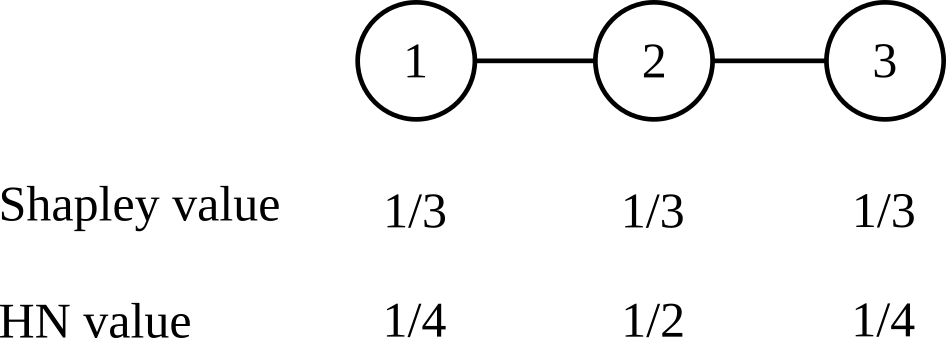
\includegraphics[scale=1.7]{shapley_hn_example.png}
    \caption{Shapley values and HN values for the unanimity game $(\{1, 2, 3\}, v_{\{1, 2, 3\}}, \{\{1, 2\}, \{2, 3\}\})$ 
            with communication structure given by the shown graph.}
    \label{fig:shapley_hn_example}
\end{figure}


One approach of adapting the Shapley value to incorporate the graphical 
structure is by using the communication graph $g$ to create a partition 
$S/g \coloneqq \{\{ i \in S| i \rightarrow j\} | j \in S\}$ of a coalition 
$S$. This partition is subsequently used to transform the game with 
communication structure $(N, v, g)$ to a game without communication structure 
$(N, v/g)$ where the value is given by the sum of the values $v$ for each component\cite{hamiache_value_1999}


\begin{equation}
    (v/g)(S) = \sum_{R, R \in S/g} v(R). 
\end{equation}


The solution $\psi$, known as the Myerson value, is then given by the Shapley value of the 
transformed game\cite{hamiache_value_1999} 


\begin{equation}
    \psi(N, v, g) = \phi(N, v/g)
\end{equation}


However, the Myerson value is based on a questionable axiom, which states that 
when the edge between players $i$ and $j$ is broken, then the difference between 
the old value and the new value must be the same for both players 


\begin{equation}
    \psi_i(N, v, g) - \psi_i(N, v, g \setminus \{i, j\}) = \psi_j(N, v, g) - \psi_j(N, v, g \setminus \{i, j\}).
\end{equation}


This reasoning does not hold in a chemical concept as the presence and absence 
of a chemical bond has an influence on the overall electronic structure 
of the molecule, which determines the molecular properties.\cite{atkins2011molecular} 
Another criticism is that the Myerson value satisfies the equal treatment 
property for unanimity games $(N, u_R, g)$\cite{hamiache_value_1999}


\begin{equation}
    \psi_i(N, u_R, g) = \begin{cases}
        \frac{1}{|R|} & \text{ if } i \in R \\
        0 & \text{ else }
    \end{cases}.
\end{equation}


So the Myerson values for the example game is also $1/3$ for each player just 
like the Shapley value.


\subsection{Hamiache-Navarro value}


The Hamiache-Navarro value is based on the concept of an associated game.
Since a communication structure limits player communication, a coalition 
$S \subseteq N$ can only directly interact with its connected neighbors 
$\mathcal{N}(S) \coloneqq \{ j \in N \setminus S | \exists i \in S \text{ such that } \{i, j\} \in g \}$
and the connections between the neighbors are of no importance as they are not 
visible form the perspective of coalition $S$. 
For example, player one can only interact directly with player two and not with player three
in the example game.
Then, a coalition $S$ can value its own payoff $v^*(S)$ as its payoff $v(S)$ in the original game and a fraction 
$\tau$ of the net payoff obtained by cooperating with each of its connected 
neighbors separately \cref{eq:associated_game}.\cite{hamiache2001associated}
This results in a series of associated games $(N, v^*, g), (N, v^{**}, g), \dots$, 
that eventually converges to a limit game $(N, \tilde{v}, g)$. The Hamiache-Navarro 
(HN) value is then given by the payoff $\tilde{v}$ of the limit game. Note that for 
the example game, the associated payoff of player one is only directly influenced 
by player two because player one and three cannot directly communicate 
with each other. This means that the coalition $\{1, 3\}$ has a weight of zero for the 
HN value of player one. However, the Shapley value would consider the coalition 
$\{1, 3\}$ for a weight of
$\frac{|S|! ( |N| - |S| - 1)!}{|N|!} = \frac{2! (3 - 2 - 1)!}{3!} = \frac{1}{3}$ (see \cref{eq:Shapley}).


\begin{equation}
	\label{eq:associated_game}
	v^*(S) =
	\begin{cases}
		\displaystyle
        v(S) + \tau \sum_{j \in \mathcal{N}(S)} \left[ v(S \cup \{j\}) - v(S) - v(\{j\}) \right] & \text{if } |S/g| = 1 \\
		\displaystyle
		\sum_{R \in S/g} v^*(R)                                                                   & \text{otherwise}
	\end{cases}
	.
\end{equation}


If a coalition $S$ contains isolated subgraphs, the associated payoff $v^*(S)$ 
is calculated as the sum of the associated payoffs of each component $R$ in the 
coalition $S$. One component is a subgraph that does not have any isolated players. 
The set of all components $S/g \coloneqq \{\{ i \in S| i \rightarrow j\} | j \in S\}$ 
is a partition of the coalition.


The algorithm for calculating the HN value can be implemented using a matrix approach.
To be consistent, an order of the matrix columns and rows are defined. Therefore a lexicographic order is defined
for coalitions of the same size. Suppose $A$ and $B$ are coalitions of the same size where the elements are ordered
from small to large (i.e. $a_1 < a_2 < \dots < a_k, \quad a_i \in A$). The coalition $A$ comes lexicographic
before coalition $B$ ($A \prec B$) if and only if $a_1 < b_1$ or $\exists \gamma \in \mathbb{N}, 1 \le i < \gamma: a_i = b_i \land a_\gamma < b_\gamma$.
For two arbitrary coalitions $S$ and $T$, $S < T$ if $|S| < |T|$ or $S \prec T$. 
Using this ordering, the characteristic function $v$ of the game $(N, v, g)$ 
can be represented as a vector in $\mathbb{R}^{2^N - 1}$, where the first $|N|$ elements 
correspond to the values of coalitions of size one, the next $\frac{|N|!}{2!(|N| - 2)!}$, etc . 
For the running example, this results in the following characteristic vector:


\begin{equation}
    \begin{aligned}
        v &= \begin{pmatrix}
        v(\{1\}) & v(\{2\}) & v(\{3\}) & v(\{1, 2\}) & v(\{1, 3\}) & v(\{2, 3\})& v(\{1, 2, 3\})
    \end{pmatrix}^T \\
    &= \begin{pmatrix}
      0 & 0 & 0 & 0 & 0 & 0 & 1
    \end{pmatrix}^T 
    \end{aligned}
\end{equation}


The associated game
\cref{eq:associated_game} $v^*_\tau = P_g M_c P_g v$ can then be written as a linear transformation of the characteristic vector
, where the square matrix $M_c$ for two arbitrary coalitions $\emptyset \ne S \subseteq N$
and $\emptyset \ne T \subseteq N$ is given by\cite{hamiache_associated_2020,hamiache2010matrix}


\begin{equation}
	M_c[S, T] =
	\begin{cases}
		1 - |N \setminus S| \tau & \text{if } |S| = |T|                         \\
		\tau                     & \text{if } |S| + 1 = |T| \land S \subseteq T \\
		-\tau                    & \text{if } |T| = 1  \land T \not \subseteq S \\
		0                        & \text{otherwise}
	\end{cases}
\end{equation}


and matrix $P_g$ is given by

\begin{equation}
	P_g[S, T] =
	\begin{cases}
		1 & \text{if } T \in S/g \\
		0 & \text{otherwise}     \\
	\end{cases}
	,
\end{equation}


which represents the graphical structure of the game. This allows to write the series of associated
games as $v^*_\tau = P_g M_c P_g v, v^{**}_\tau = P_g M_c P_g v^*_\tau, \dots, v^{(k*)}_\tau = \left(P_g M_c P_g\right)^k v$.
Provided that $\tau$ is small enough ($\tau < \frac{2}{|N|}$ for complete graphs\cite{hamiache2001associated}),
the power series $\left(P_g M_c P_g\right)^k v$ converges as $k$ tends to infinity.\footnote{A proof can be found in \cite{hamiache_associated_2020}}
The convergence produces a limit game $(N, \tilde{v}, g)$, where the solution $\phi_i$ of player $i$ equals the
payoff $\tilde{v}(\{i\})$ of player $i$.\cite{zhang2022gstarx, hamiache_associated_2020}
Matrices for the example game are given in \cref{app:HN_example}.


% \textbf{Numerical example}
% 
% In order to compare the Hamiache-Navarro value and the Shapley value the same example as in \cref{subsec:shapley_value}
% is used. To recap, define an unanimity game with communication structure $(\{1, 2, 3\}, u_{\{1, 2, 3\}}, \{\{1, 2\}, \{2, 3\}\})$
% where $u_{\{1, 2, 3\}}(S)$ is one if $\{1, 2, 3\} \in S$ and zero otherwise with $S \subseteq \{1, 2, 3\}$. As discussed
% in \cref{subsec:shapley_value}, the Shapley value is equal to $1/3$ for all players. However, the HN-value is not equal
% for all players. Players one and three have an HN-value of $1/4$ and the HN-value for player two is $1/2$
% (see \cref{app:HN_example}).\cite{hamiache_associated_2020}

\chapter{Methodology}


\section{Data set description}


MoleculeNet provides publicly available benchmark data sets for the prediction of 
various molecular properties.\cite{wu2018moleculenet} Here, the ESOL data set is used,
which contains the measured solubility at $25^{\circ} C$ in $log(mol/L)$ for $1110$ 
distinct small molecules, each represented as a SMILES string. 
From this representation various chemical properties can be computed using the RDKit python package\cite{landrum2010r}. 
The following properties are used to create the node feature vector: \cite{wu2023chemistry}

\begin{itemize}
    \item \textbf{Atom symbol:} One hot encoding of the atom type \\
        $\left( [B, C, N, O, F, Si, P, S, Cl, As, Se, Br, Te, I, At, metal] \right)$
    \item \textbf{Degree:} Number of covalent bonds (minimum is $0$ and maximum is $5$)
    \item \textbf{Formal charge:}\cite{parkin2006valence} The formal charge of an atom is defined as the difference between its valence 
        electrons and the number of electrons assigned from the Lewis structure where each single bond 
        contributes one electron. For example, nitrogen $(N)$ in nitrobenzene (\cref{fig:nitrobenzene})
        has a formal charge of $+1$, because $N$ has five valence electrons and gets four electrons 
        from the Lewis structure (one electron from each of the single bonds and two from the double bond).

        \begin{figure}[h]
            \centering
            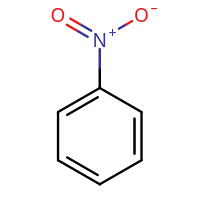
\includegraphics[scale=0.5]{nitrobenzene.png}
            \caption{Lewis structure of nitrobenzene}
            \label{fig:nitrobenzene}
        \end{figure}

    \item \textbf{Hybridization:}\cite{alabugin2015orbital} One hot encoding of the orbital structure of the atom \\
        ($[sp, sp^2, sp^3, sp^3d, sp^3d^2, other]$)

    \item \textbf{Aromaticity:} An aromatic system is a ring containing a delocalized electron 
        structure with $4n + 2$ electrons. For example, the benzene ring in \cref{fig:nitrobenzene}
        is an aromatic structure. ($0$ or $1$)

    \item \textbf{Hydrogens:} Hydrogen atoms are treated implicitly in order to prevent the
        explosion of the number of nodes in a molecular graph. If hydrogen atoms 
        were treated explicitly, then nitrobenzene (\cref{fig:nitrobenzene}) would 
        already have five more nodes, increasing the total nodes from ten to fifteen.
        (One hot encoding: $[0, 1, 2, 3, 4]$)

    \item \textbf{Chirality:}\cite{prelog1976chirality} Indicates whether the atoms is a chiral center. Chirality 
        occurs when for example a carbon atom is bonded to four different groups. 
        Then the spatial orientation of those groups matters as not all configurations 
        are equivalent under rotation. ($0$ or $1$)

    \item \textbf{Chirality type:} One hot encoding of the chirality type $([R, S])$.

\end{itemize}


The type of an edge is determined by a bond feature vector consisting of the following chemical properties:


\begin{itemize}
    \item \textbf{Bond type:} One hot encoding of bond type ([single, double, triple, aromatic])
    \item \textbf{Conjugation:} Indicates whether the bond is part of a delocalized electron strucure.
        ($0$ or $1$) 
    \item \textbf{ring:} Indicates whether the bond is part of a ring ($0$ or $1$).
    \item \textbf{Stereo:} One hot encoding of stereo configuration of the bond.
        ([StereoNone, StereoAny, StereoZ, StereoE])
\end{itemize}


\section{Architecture of the graph neural network model to predict water solubility}


Prediction of water solubility is achieved using the same RGCN model as Wu et. al. (\cref{fig:ml_model}),
with the hyper parameters listed in \cref{tab:hyperparameters}. To obtain more 
robust predictions, ten models are trained, each with a different seed 
$(2023 + 10i, \text{ with } i \in \{1, 2, \dots, 10\})$, where the final 
prediction is then obtained by the average prediction over all models.\cite{wu2023chemistry} 
The model is implemented in python using PyTorch Geometric\cite{Fey/Lenssen/2019}, training progress 
is tracked using wandb\cite{wandb} and analysis of the results is done using 
pandas\cite{reback2020pandas} an plotly\cite{plotly}.


\begin{figure}[h]
    \centering
    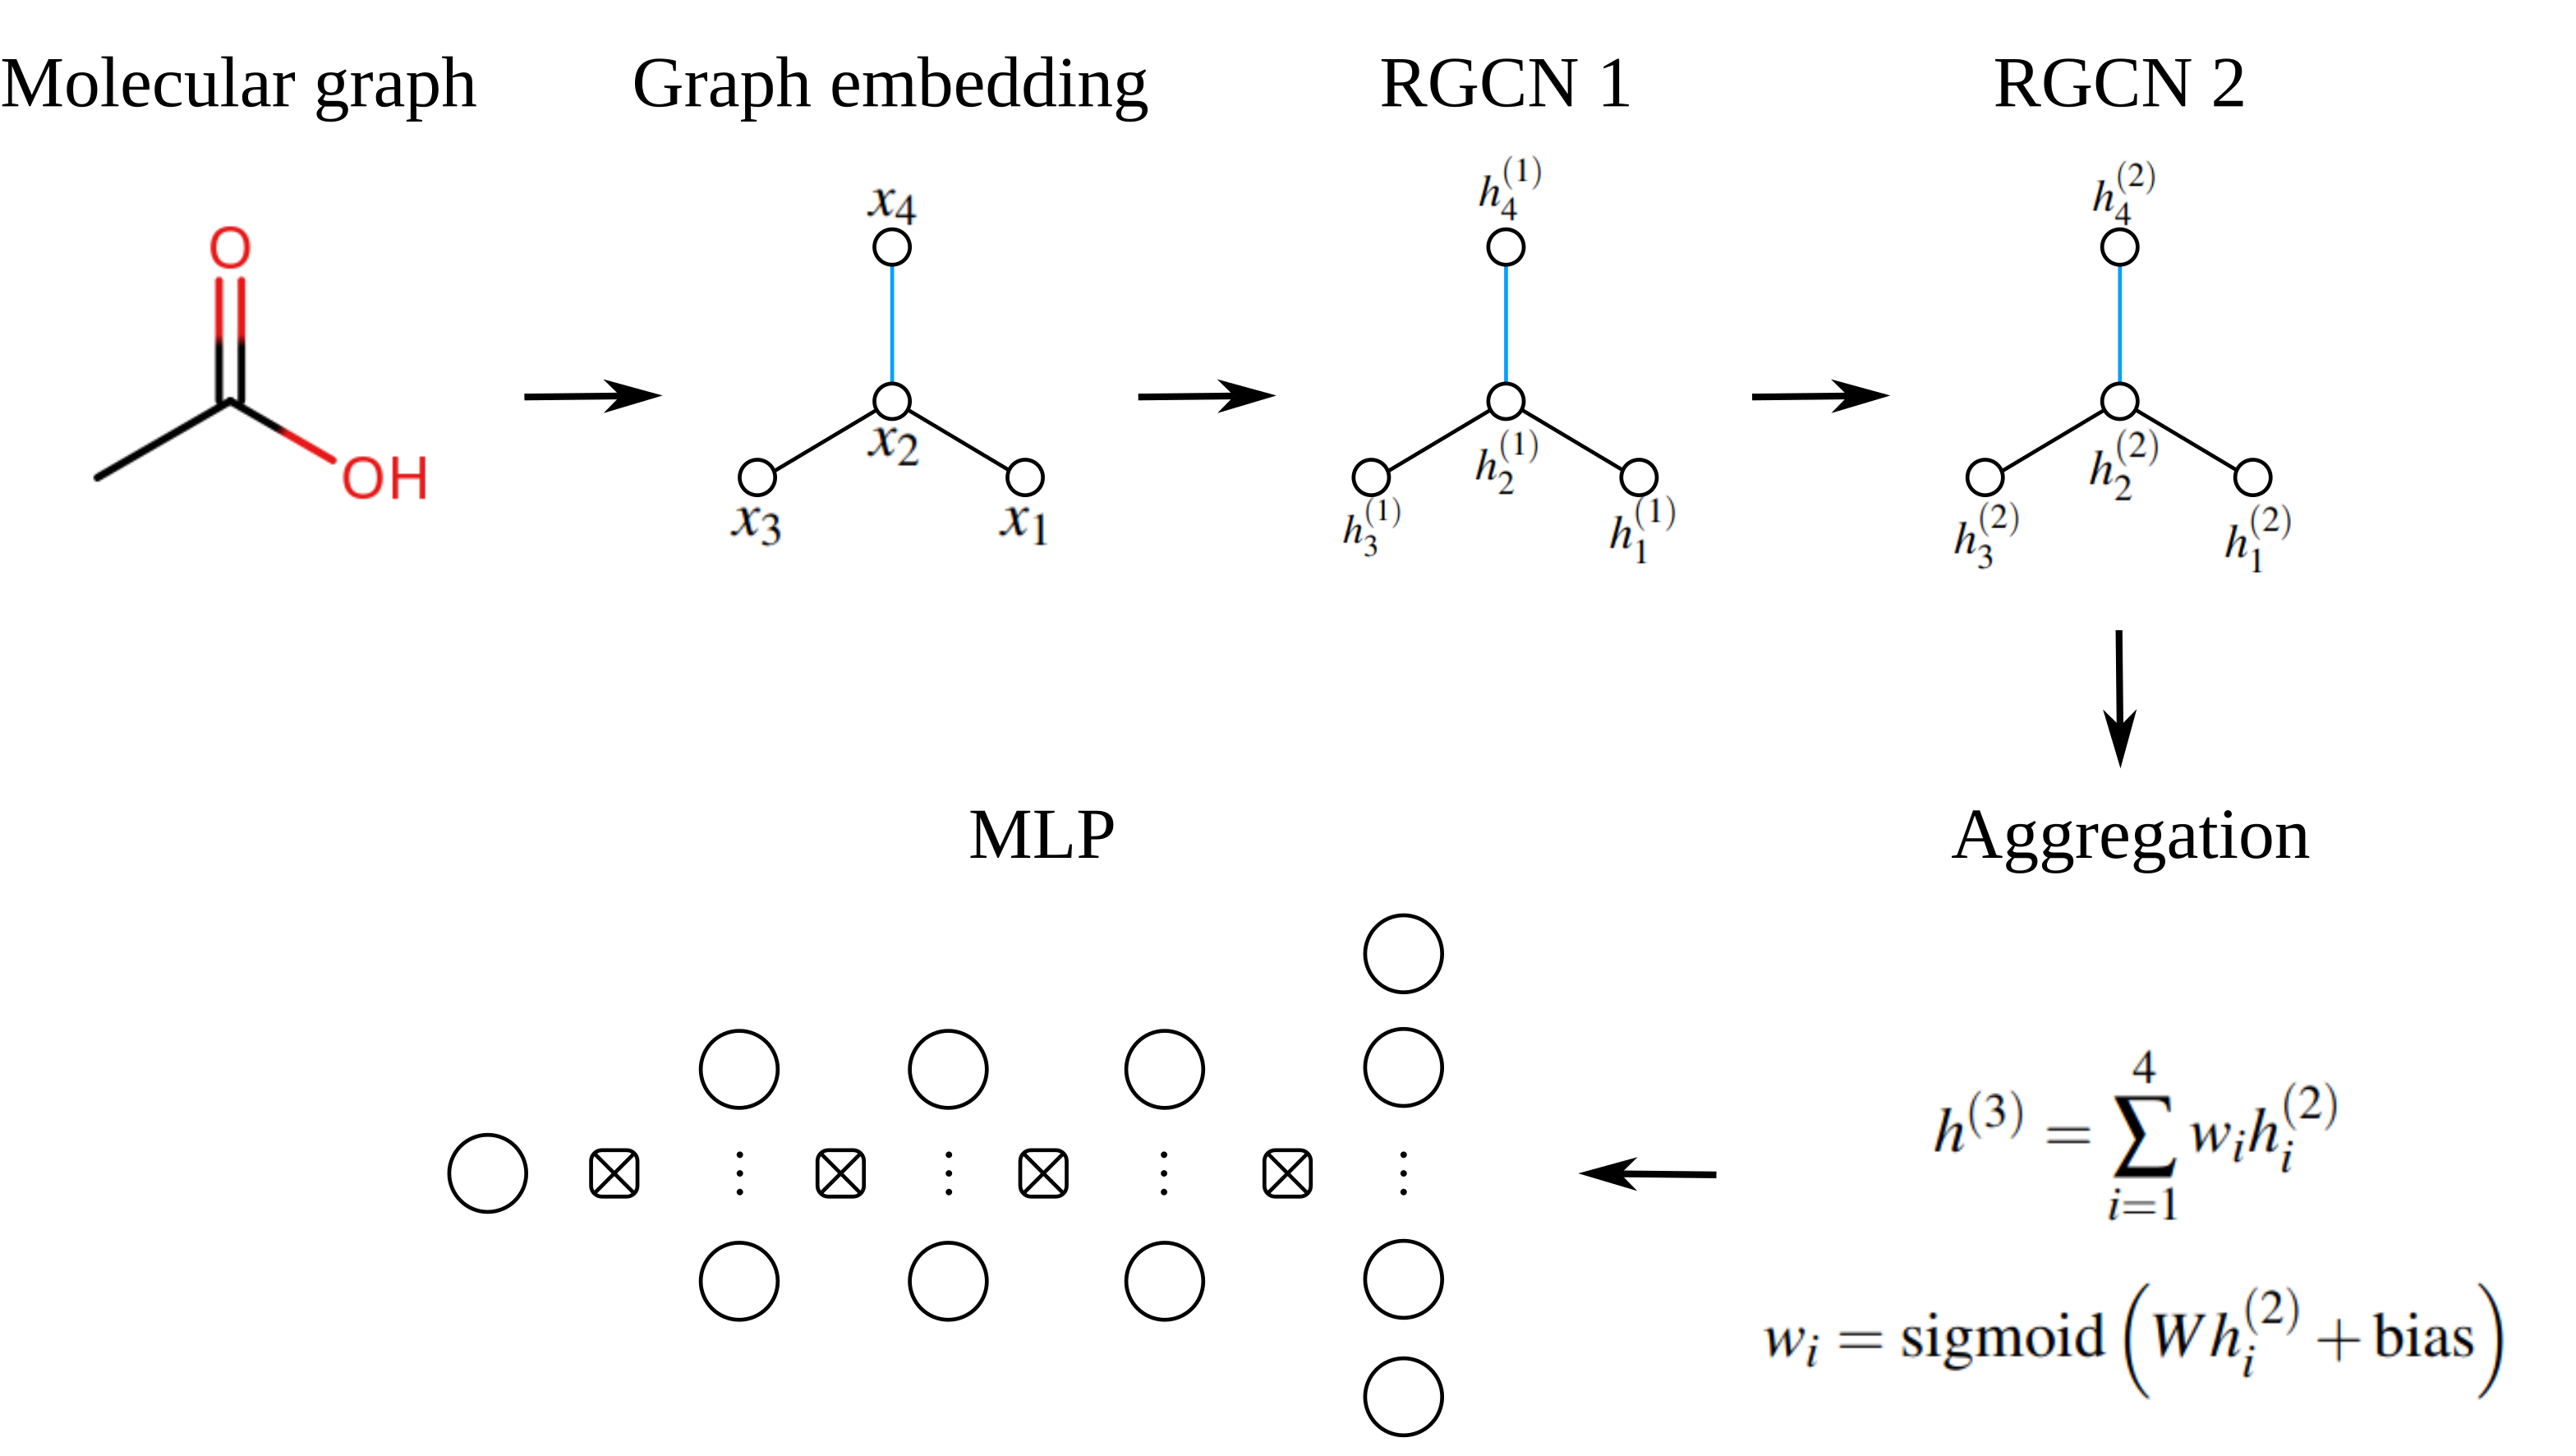
\includegraphics[scale=0.85]{rgcn_model.png}
    \caption{Machine learning model used for the prediction of water solubility of 
        small molecules. First, the molecular graph is embedded to a graph where the 
        bond features are used to determine edge types and node features are computed 
        using the RDKit python package. Next, two RGCN layers are applied, which are 
        followed by a weighted sum to aggregate the whole graph into one vector. This 
        vector is then passed to an MLP to obtain the final prediction.
    }
    \label{fig:ml_model}
\end{figure}


\begin{table}[h]
    \caption{ Hyper parameters from \protect\citen{wu2023chemistry} of an RGCN model to predict water solubility.}
    \label{tab:hyperparameters}
    \begin{center}
        \begin{tabular}{cc}
            \toprule
            \textbf{hyper parameter} & \textbf{value} \\
            \midrule
            RGCN layers & 2 \\
            RGCN hidden units & 256 \\
            RGCN dropout rate (each layer) & 0.5 \\
            MLP hidden units & 64 \\
            MLP dropout rate (each layer) & 0.1 \\ 
            Epochs & 500 \\
            Early stop & 30 \\
            \bottomrule
        \end{tabular}
    \end{center}
\end{table}



\chapter{Results and discussion}


This section first discusses the performance of the model, followed by
the comparison of the distributions of functional groups attributions computed 
using the different methods. Subsequently, agreement and disagreement between 
the attribution methods are examined using pairwise Spearman rank correlation. 
Next, agreement between attributions and chemical expectations is analyzed. 
Finally, the faithfulness of the attribution methods to the model is assessed 
using the fidelity metric.

 
\section{RGCN is able to accurately predict expected water solubility}


The resulting ten RGCN models, each with a different seed, have comparable results 
(\cref{fig:training_history}). 
Performance of the training data is relatively good, yielding an average $R^2$ 
of $0.9630$ and an average mean squared error (MSE) of $0.0744$ (\cref{tab:model_performance}). 
The model has a similar $R^2$ for the validation data, however, larger errors are made. 
Model performance on the test data is similar as the validation performance, showing that the 
model is able to generalize well to unseen data. Considering that most experimental data have an RMSE 
between $0.6$ and $0.7$ log(mol/L),\cite{palmer2014experimental} 
it can be concluded that the resulting model can predict water solubility of small 
molecules with decent performance.

% \begin{figure}[h]
%     \centering
%     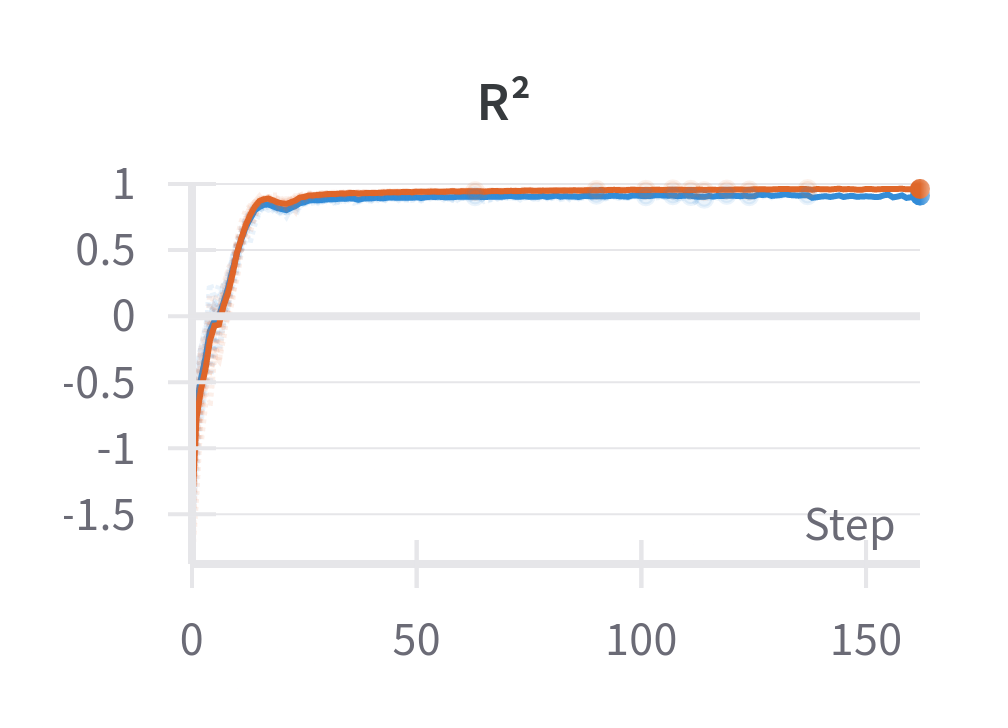
\includegraphics[scale=0.20]{rgcn_r2.png}
%     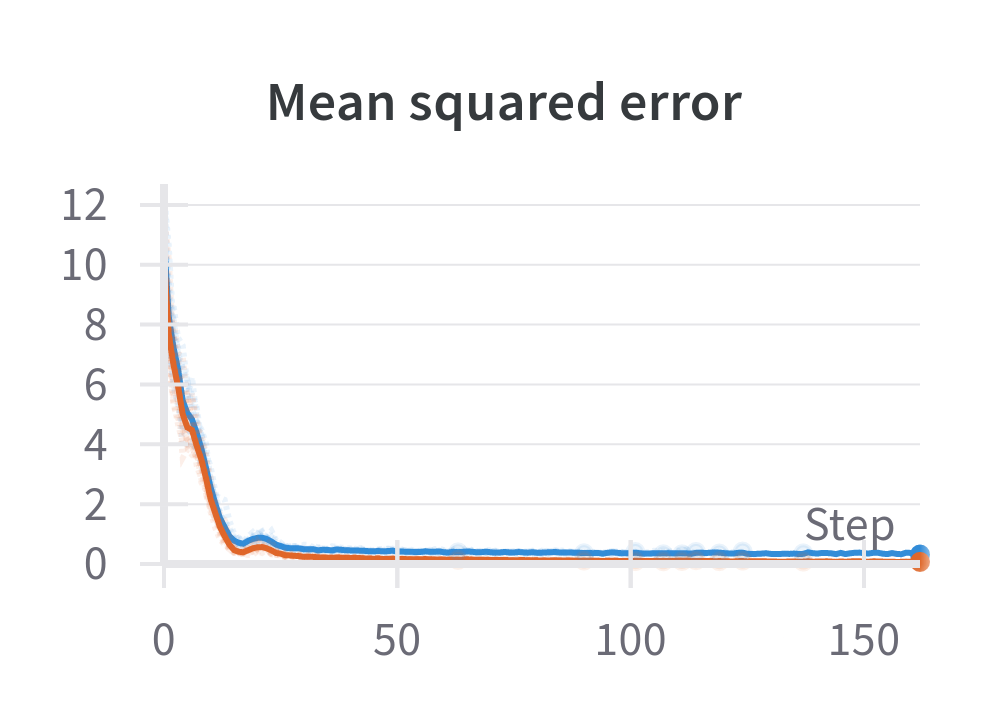
\includegraphics[scale=0.20]{rgcn_mse.png}
%     \caption{Average Mean squared error (left) and $R^2$ (right) of train (orange) and validation 
%     (blue) data during model training over the ten RGCN models, each trained using a different 
%     seed. Both metrics show a good model performance and no overfitting.}
% \end{figure}


\begin{figure}[h]
    \centering
    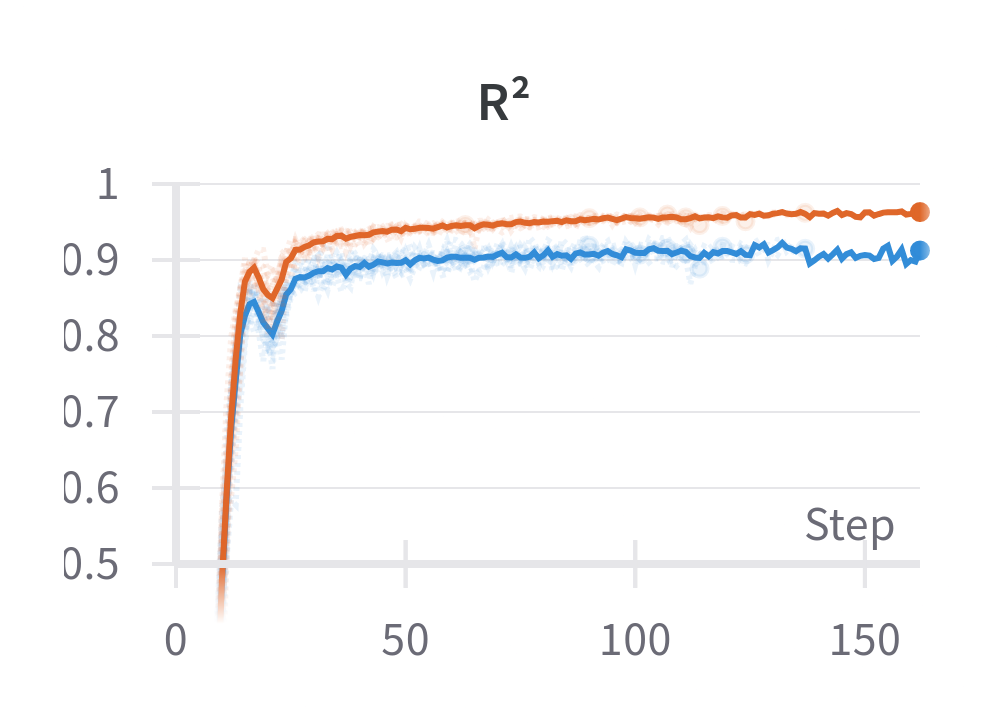
\includegraphics[scale=0.20]{rgcn_r2_zoomed.png}
    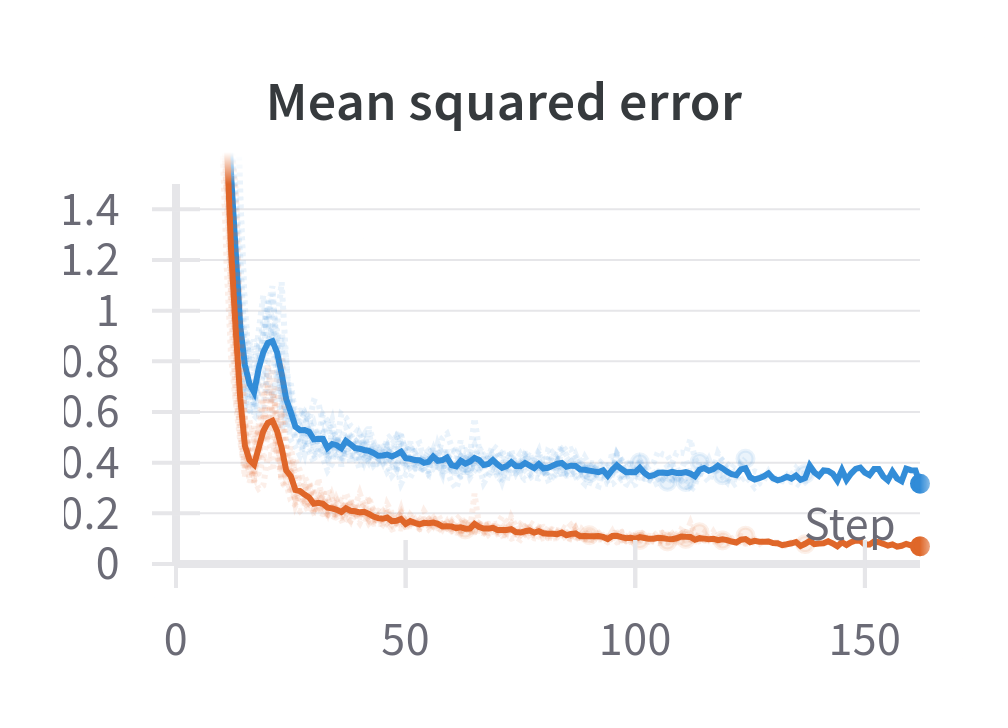
\includegraphics[scale=0.20]{rgcn_mse_zoomed.png}
    \caption{Average $R^2$ (left) and mean squared error (right) of train (orange) and validation 
    (blue) data during model training over the ten RGCN models, each trained using a different 
    seed. Both metrics show a good model performance and no overfitting. }
    \label{fig:training_history}
\end{figure}


\begin{table}[h]
    \centering
    \caption{Average $R^2$ and MSE for train, validation and test data sets with standard deviation between brackets.}
    \label{tab:model_performance}
    \begin{tabular}{ccc}
        \toprule 
       & $\pmb{R^2}$ & \textbf{MSE $\pmb{\left(\left[log(mol/L)\right]^2\right)}$} \\
        \midrule
        \textbf{Train} & $0.9630 (\pm 0.0001)$ & $0.0744 (\pm 0.0031)$ \\
        \textbf{Validation} & $0.9225 (\pm 0.0076)$ & $0.3354 (\pm 0.0120)$ \\
        \textbf{Test} & $0.9079 (\pm 0.0050)$ & $0.3193 (\pm 0.0047)$ \\
        \bottomrule 
    \end{tabular}
\end{table}



Currently, it is questionable whether the ML model effectively learns chemistry and 
if wrong predictions may be explained by chemically incorrect reasoning of the model. 
To address this, different attribution methods (SME, Shapley value and HN value) are 
compared to each other and with chemical theory. It should be noted that these attribution 
methods can reveal insights into the chemical reasoning of the model, but are not necessarily 
causal. This means that if the attributions show inconsistency with chemical theory, other 
factors could also influence the wrong prediction.


\section{Different attribution methods can result in different explanations}
\label{sec:results_different_explanations}


The attribution values sign usually shows an agreement with expectations from 
chemistry (\cref{fig:attribution_distribution_fg}). Groups that positively affect the polarity of a molecule have a 
positive attribution, while unfavorable functional groups for water solubility 
have a negative attribution. The median of HN values also shows a correct 
relationship between the functional groups. Hydroxyl groups are hydrogen bond 
acceptors and donors, so it has a superior influence on water solubility than 
a methyl ester that can only accept hydrogen bonds. Also, ethoxy has a lower 
HN value than methoxy, which is due to the larger carbon chain of ethoxy.


\begin{figure}[h]
    \centering
    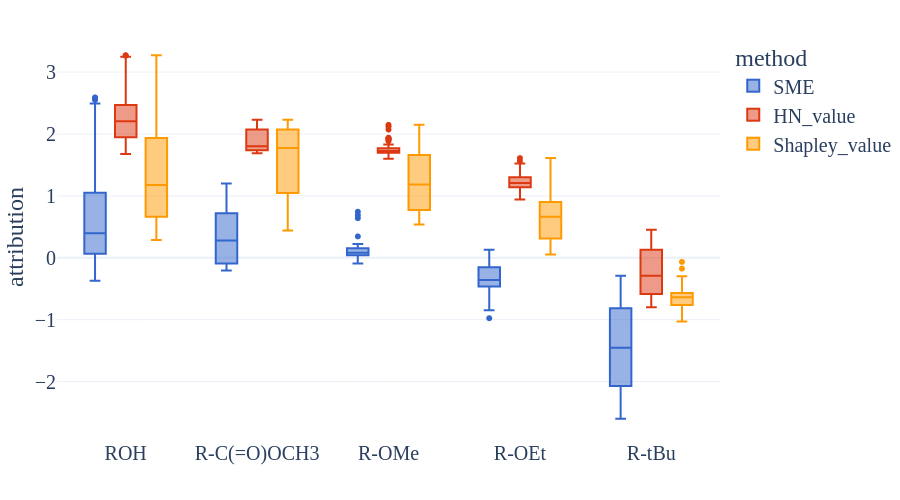
\includegraphics[scale=0.5]{attribution_distribution_functional_groups.png}
    \caption{The Shapley value, HN value, and SME attribution distributions for selected functional groups.}
    \label{fig:attribution_distribution_fg}
\end{figure}


Shapley values have mostly a broader IQR relative to the HN values. The median 
Shapley value of alcohols is lower than methyl esters, which is unexpected. 
However, SME assigns negative attributions to hydroxyl groups, which incorrectly suggests 
that hydroxyl groups can decrease the solubility of small molecules. One of those 
molecules is erythritol (\cref{fig:erythritol_explanation}), which has a predicted solubility of 0.432 log(mol/L) 
and an experimental solubility of 0.700 log(mol/L). Since the absolute prediction 
error is within acceptable limits, it would be possible that the model achieved 
this in a chemically incorrect way (i.e. clever Hans effect\cite{lapuschkin2019unmasking}). 
Clever Hans effect is a correct model prediction, however, due to the wrong reason. 
The clever Hans effect is supported by the wrong Shapley value explanation as it gives the 
apolar carbon chain a higher attribution than the hydroxyl groups. However, 
the explanation of the HN values is chemically correct, which makes it difficult 
to judge whether there is a clever Hans effect. 

Furthermore, the absolute prediction 
error for only five of the sixteen molecules with a negative SME attribution for 
hydroxyl groups is greater than the experimental error. However, those five molecules 
have a chemically consistent explanation from Shapley and HN values. The fact that only 
five of the wrong SME explanations are indeed wrongly predicted and the other attribution 
are in agreement with chemical theory tends to show that SME does not provide the correct 
model explanation. To obtain better understanding of the agreement/disagreement between 
attribution methods and the relation with absolute prediction error, a ranked based analysis is performed. 


\begin{figure}[h]
    \centering
    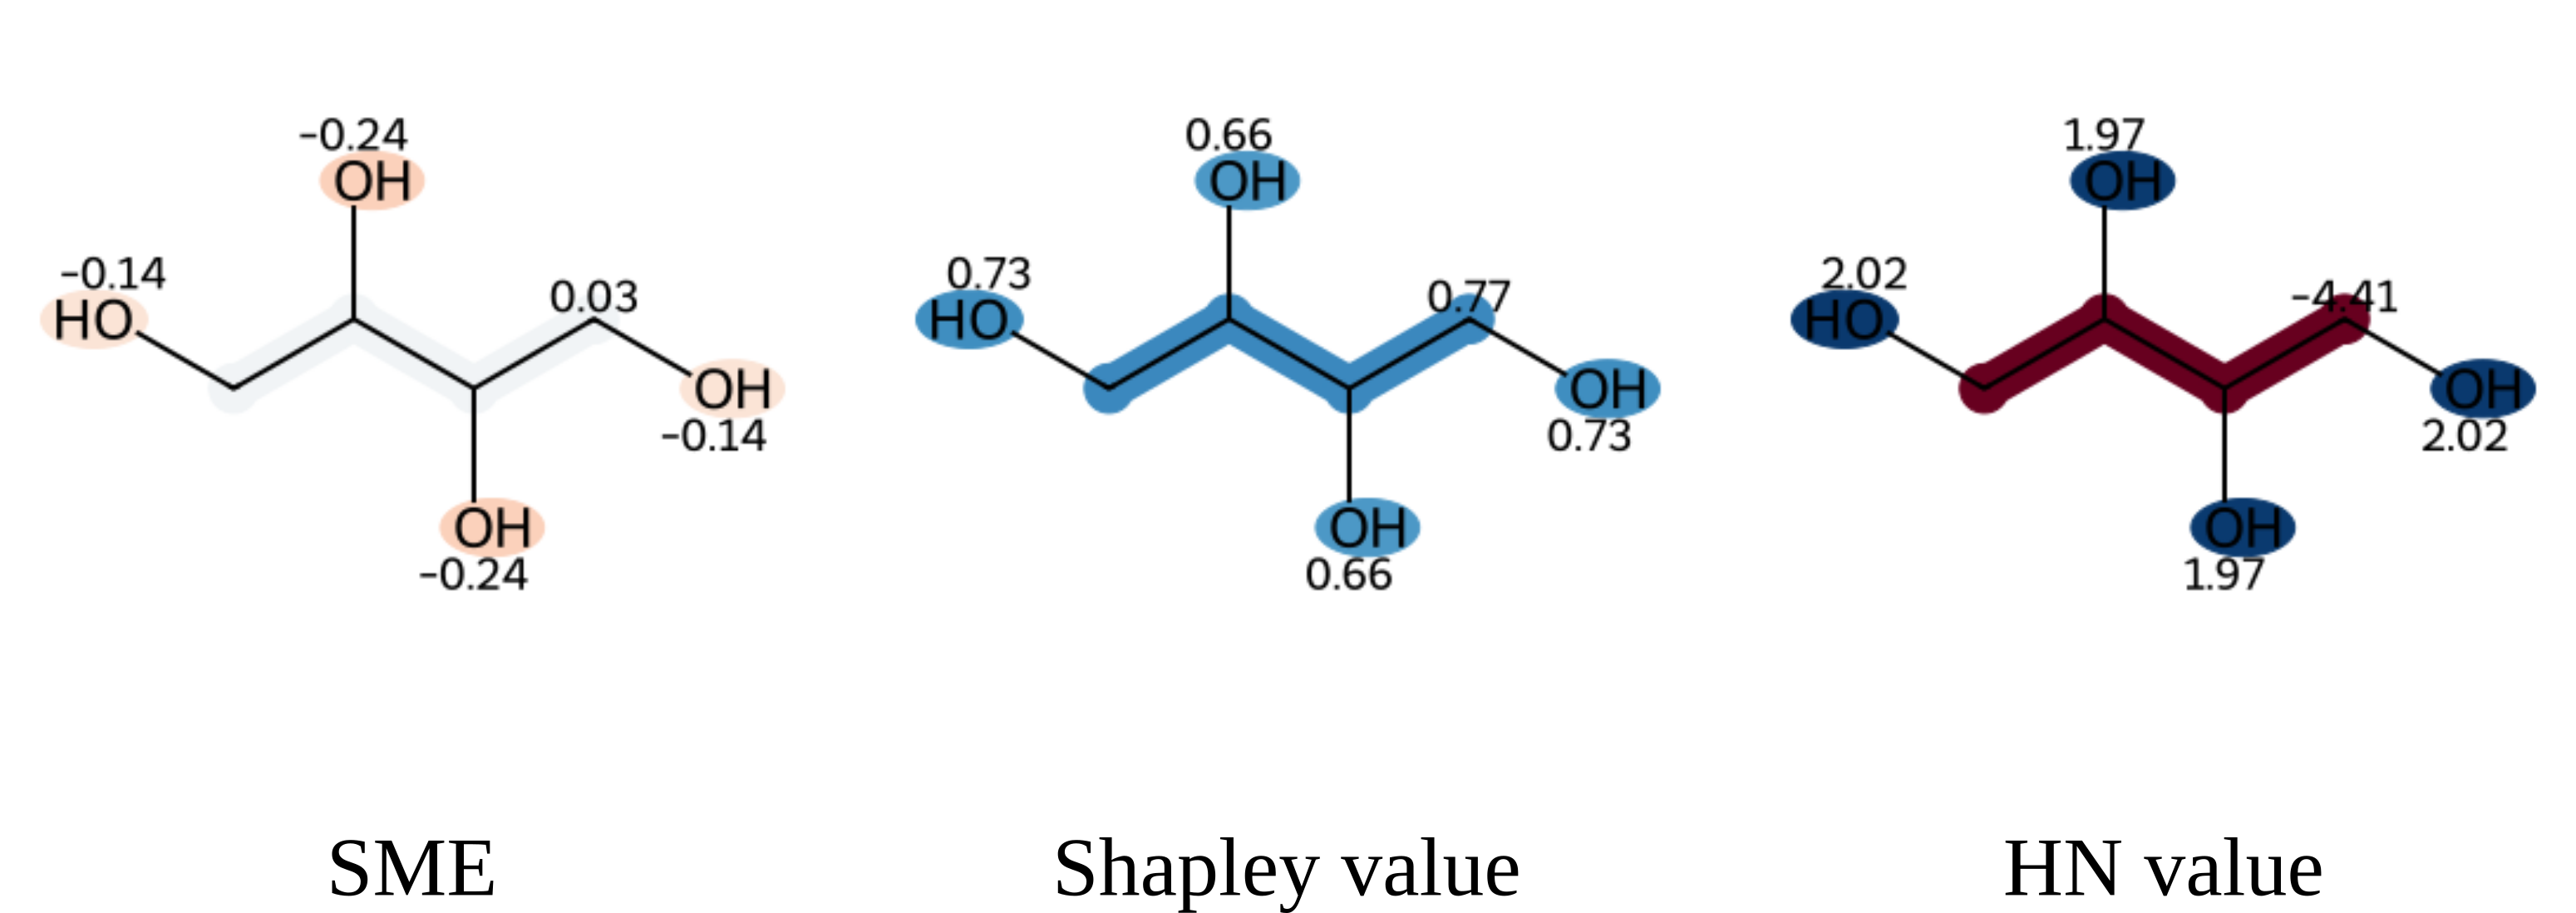
\includegraphics[scale=0.85]{erythritol_explanations.png}
    \caption{Explanations of erythritol: SME is wrong due to the negative attributions on the hydroxyl groups, 
    Shapley values are wrong since hydroxyl groups have a lower attribution than the carbon chain, HN values provide 
    a chemically correct explanation. Predicted solubility is 0.432 log(mol/L) and the experimental water solubility is 
    0.700 log(mol/L).}
    \label{fig:erythritol_explanation}
\end{figure}


\section{Absolute prediction error is not associated with the Spearman rank correlation between different attribution methods}


To get more insight into agreement or disagreement between attribution methods
and whether disagreement can be explained by the absolute prediction 
error, a ranked based approach is used. For each molecule, the substructures are ranked  
from most negative (i.e. most hydrophobic) towards most positive (i.e. most hydrophylic). 
Subsequently, the Pearson correlation is computed between the ranks of two attribution methods.


SME and Shapley value attribution rankings agree most often with each other, $78.07\%$
of the molecules have a Spearman rank correlation of one. Two molecules have 
a complete opposite explanation, where the chemically correct ranking is provided by the 
Shapley value based ranking. Overall, no association is observed between Spearman 
correlation and the absolute prediction error. 


Perfect agreement between HN value and Shapley value ranks happens for 
$74.26\%$ of the molecules. Again at low correlation $( \le -0.5)$, the ranking based on 
the Shapley value is most often chemically correct. Also no association between prediction error 
is observed, showing that the addition of graphical structure in the explanation 
method does not systematically change the explanation.


 

\begin{figure}[h]
    \centering
    % 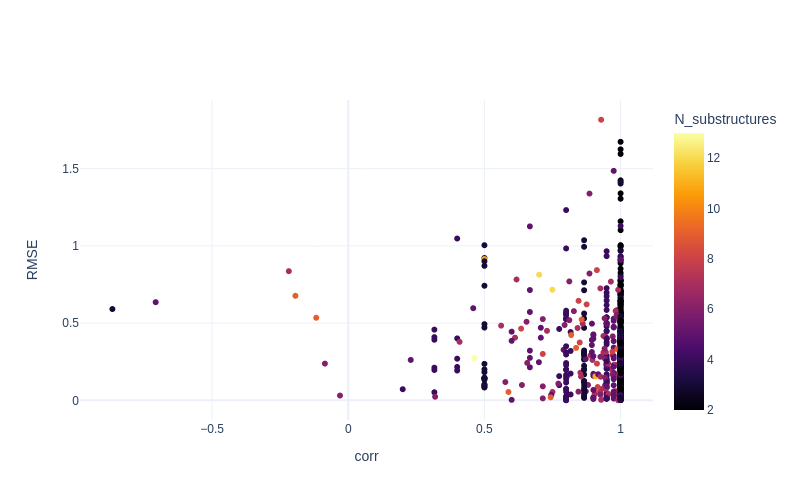
\includegraphics[scale=0.35]{../data/images/esol_rank_vs_AE_SME_Shapley_combined.png}
    % 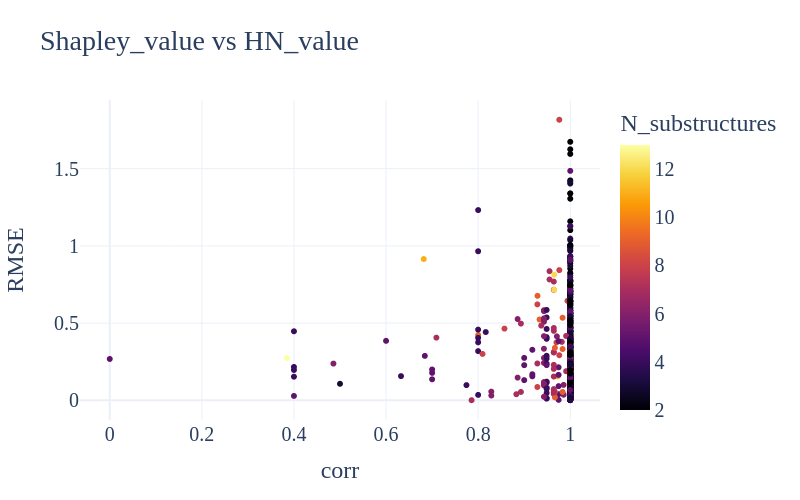
\includegraphics[scale=0.35]{../data/images/esol_rank_vs_AE_Shapley_HN_combined.png}
    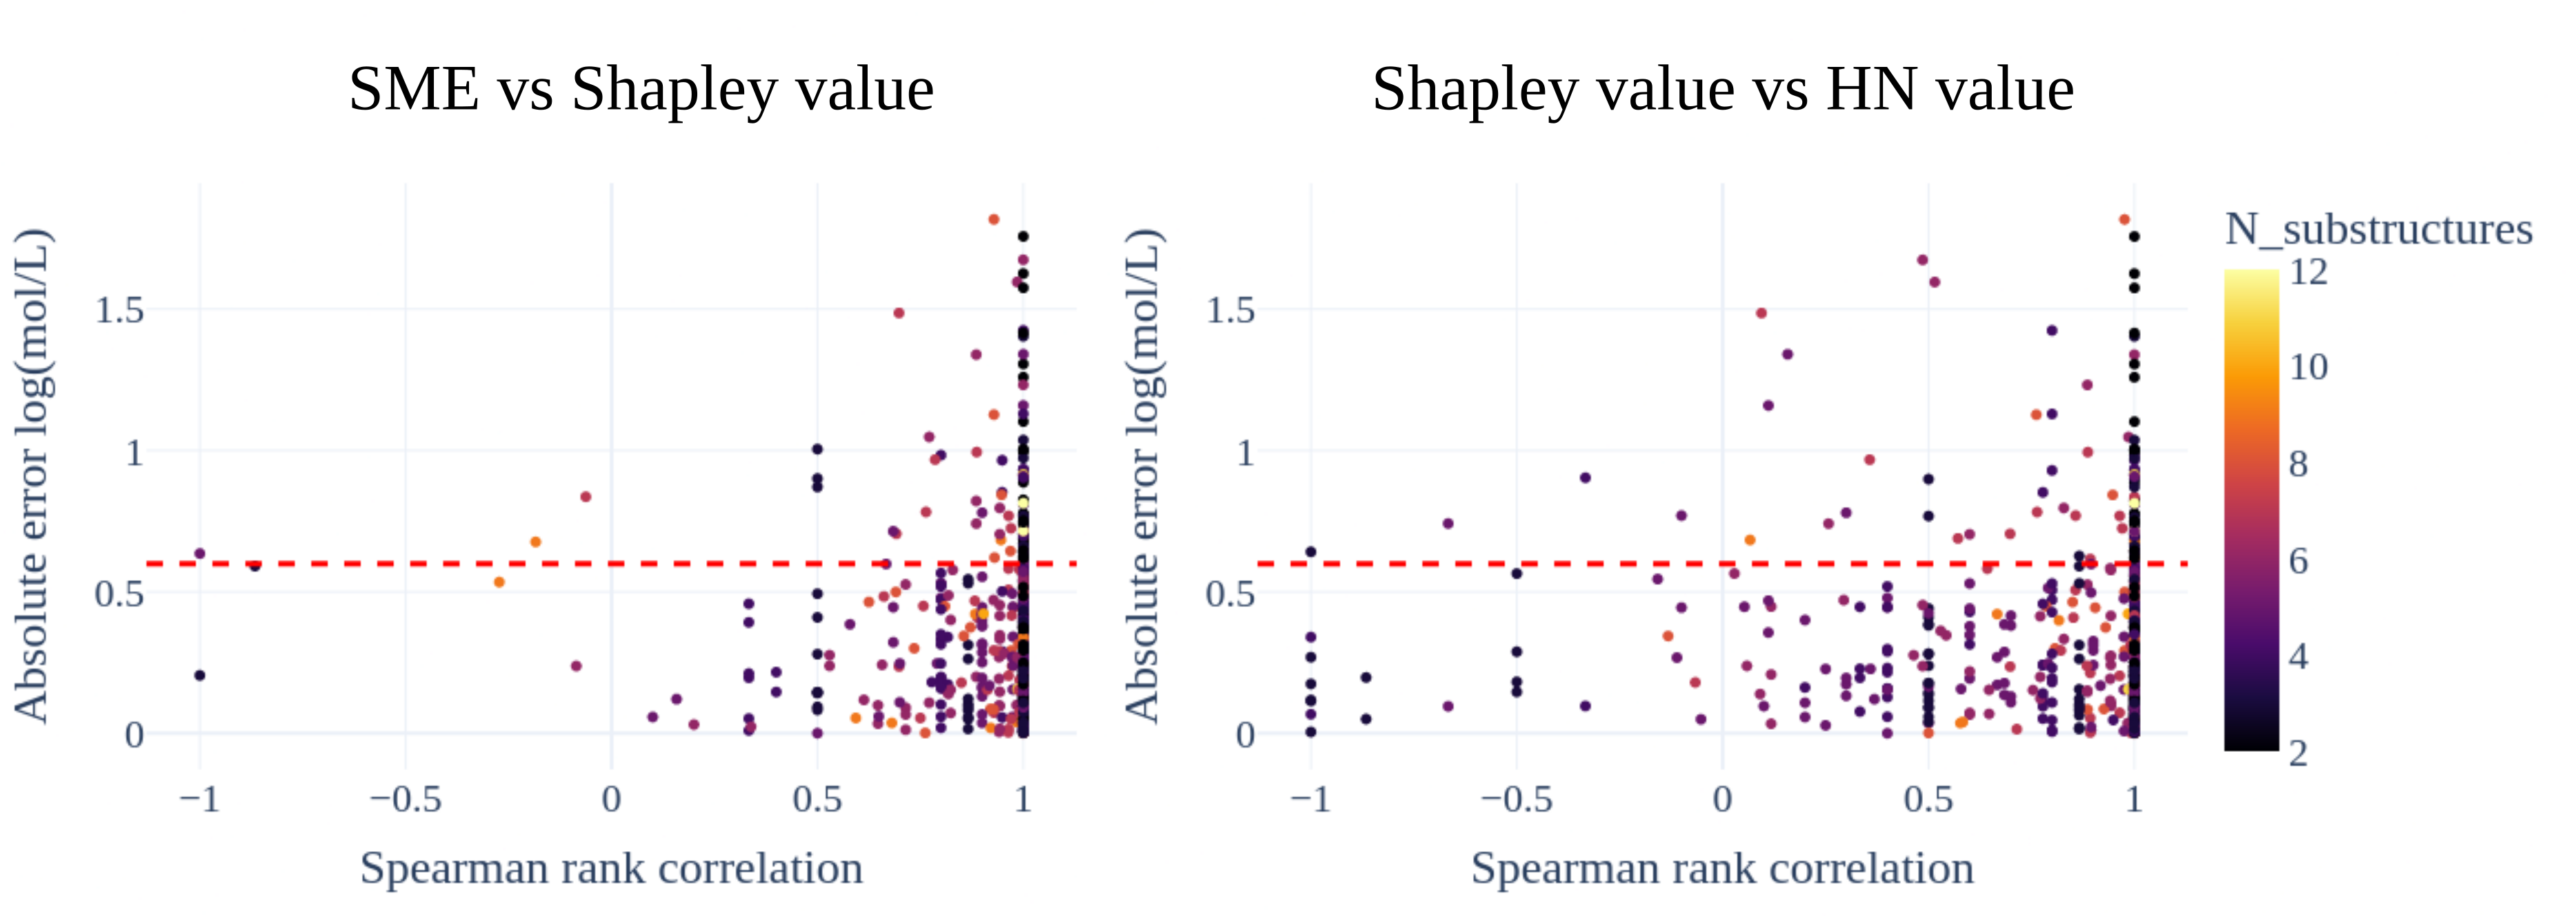
\includegraphics[scale=0.75]{rmse_vs_rank_corr_attributions.png}
    \caption{Absolute error of model prediction in function of Spearman rank correlation between 
        attributions from SME and Shapley (left) and between Shapley and HN (right) using the full 
        data set containing 1110 molecules. The red line shows experimental error of 0.6 log(mol/L).
    }
\end{figure}


\section{All attribution methods have a similar ranking with chemical expectations}

% \section{Relative evaluation of attribution methods using chemically intuitively ranked substructures shows no statistical
% significant difference between the attribution methods}


To analyze which attribution method provides the most accurate
explanation, the Spearman rank correlation is computed between the
substructures attributions and a chemically intuitive ranking of those
substructures for $100$ molecules from the test data set. Also the influence of the absolute error between model
prediction and experimental value is examined by subdividing the
molecules into two error groups based on experimental error $(<0.6 \text{ or } >=0.6)$. Since the distributions of
the Spearman rank correlations are highly skewed to the left,
non-parametric tests are used for the analysis (\cref{fig:spearman_corr_manual}). To test whether there is
a significant difference of agreement with chemical expectations between 
the different attribution methods, two Friedman tests are applied (one for each absolute error
category). Analysis of the absolute error (AE) groups for each of 
the attribution method is done using three Wilcoxon--Mann--Whitney tests.
Multiple testing is controlled by means of the Bonferonni correction, 
resulting in a significance level of $0.05/5 = 0.01$.


\begin{figure}[h]
    \centering
    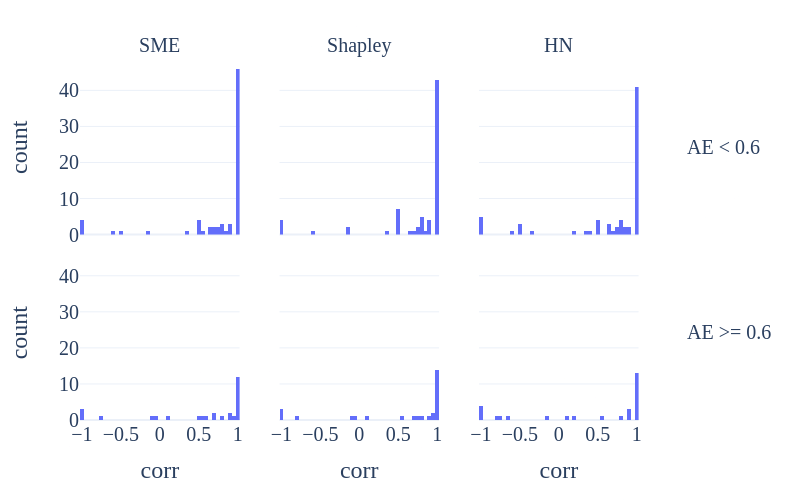
\includegraphics[scale=0.5]{spearman_rank_correlation_manual_vs_attribution.png}
    \caption{Distribution of Spearman rank correlation between an attribution method 
        and a manual ranking of substructures using chemical reasoning. The difference 
        between the two absolute error groups is mainly the intensity of high 
        correlation values.
    }
    \label{fig:spearman_corr_manual}
\end{figure}


The presence of a statistically significant difference in Spearman rank correlation
between attributions and chemically intuitive ranks for different
attribution methods is tested using a Friedman test. The null-hypothesis
assumes that there is no difference between the different attribution
methods, which would result in similar rank sums of the different
attribution methods. When the absolute prediction error is below the 
experimental error, then no statistical significant difference between 
the different attribution methods is observed (p-value $0.0154$) based 
on the Bonferonni corrected nominal level of $0.01$(\cref{fig:friedman_results}). 
Also when the absolute prediction error is above the experimental error, no significant difference 
is present between the different attribution methods (p-value $0.0148$). 
Therefore, we conclude that there is not enough
evidence in the data to reject the null hypothesis. However, considering 
that the current sample size equals $100$ and the p-values are close to the 
nominal level, it is recommended to confirm these findings in a follow up 
study with a larger sample size.


\begin{table}[h]
    \centering
    \caption{Average Spearman rank correlation between chemically ranked substructures and 
    a ranking based on attribution values.}
    \begin{tabular}{cccc}
    \toprule
    AE & SME & Shapley & HN \\
    \midrule
     < 0.6 & 0.7767 & 0.7708 & 0.6891 \\
    $\ge$ 0.6 & 0.5136 & 0.5482 & 0.3732 \\
     \bottomrule
    \end{tabular}
\end{table}


\begin{table}[h]
    \centering
    \caption{Friedman test results}
    \label{fig:friedman_results}
    \begin{tabular}{ccccc}
    \toprule
    AE & N & Statistic & df & p \\
    \midrule
     < 0.6 & 72 & 8.348 & 2 & 0.0154  \\
    $\ge$ 0.6 & 28 & 8.432 & 2 & 0.0148 \\
     \bottomrule
    \end{tabular}
\end{table}



In all attribution methods there is no significant difference between the two different
absolute error groups (p-values are $0.0214$, $0.1694$, $0.0789$ for SME, Shapley and
HN respectively). Therefore, we conclude that there is not enough evidence in the
data to reject the null hypothesis of equal distributions. 

% In other words, no attribution 
% method has a higher disagreement with chemical expectations when the prediction error 
% is above experimental error.


\section{All attribution methods are equally faithful to the ML model}


So far, different attribution methods have been compared in a more qualitative way. 
This is due to the difficulty of quantifying how correct an explanation is. The 
Spearman rank correlation between attribution and chemical expectation is one 
possible way to check the accuracy of the explanation. However, this raises the 
question whether the explanation is faithful to the model. It could be possible 
that an attribution method gives a chemically correct explanation but may not be 
representative of the model. 


Overall, all attribution methods posses a rather poor fidelity (\cref{fig:fidelity} and \cref{fig:absolute_fidelity}). 
The negative-fidelity has a median around $1.84 log[mol/L]$ for each attribution method when the absolute 
prediction error is below the experimental error. However, the distribution is rather 
broad and includes zero, meaning that sometimes removing the most negative attribution 
does not have an impact on the prediction. When the absolute prediction error is above 
the experimental error, the median negative-fidelity decreases to around $-2.40 log[mol/L]$, 
however the distribution is also more spread out. 


Similarly, the positive-fidelity is distributed around zero meaning that the removal of 
the most hydrophilic substructure does not have a significant effect on the predicted 
water solubility. A possible explanation for this is when multiple hydrophilic substructures 
are present, then it is possible that when one functional group is removed the solubility 
does only slightly decrease. 

The low-absolute-fidelity is smaller when the attribution is closer to zero, as expected (\cref{fig:absolute_fidelity}).
However, major changes in the predicted water solubility are observed even at low absolute 
attribution values. This shows that the attribution methods are not always faithful to the model. 


\begin{figure}[h]
    \centering
    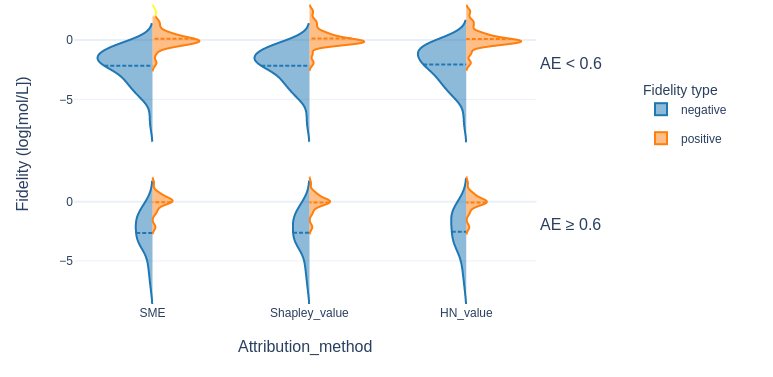
\includegraphics[scale=0.5]{fidelity_2.png}
    \caption{Distribution of fidelity obtained by removing the most positive 
        attribution (right side) or the most negative attribution (left side).
        Fidelity is computed for 100 molecules from the test data set.
    }
    \label{fig:fidelity}
\end{figure}


\begin{figure}[h]
    \centering
    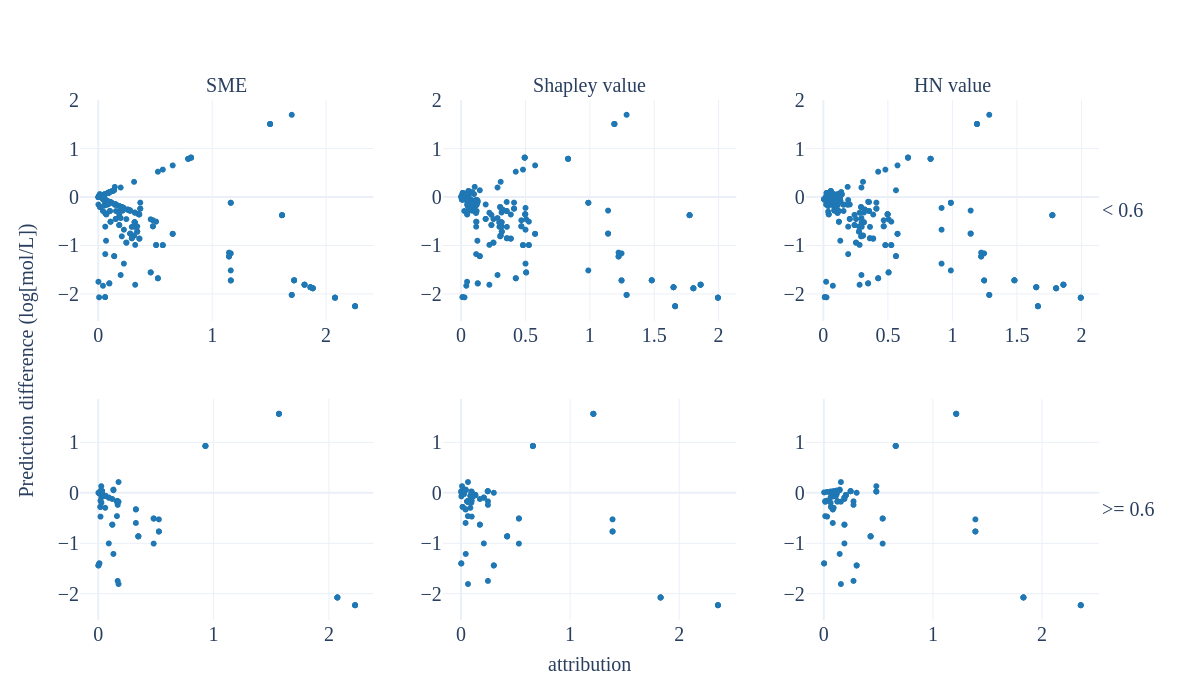
\includegraphics[scale=0.35]{absolute_fidelity_3}
    \caption{Fidelity obtained by removing the substructure 
        with the lowest absolute attribution in function of the smallest absolute attribution value.
        Fidelity is computed for 100 molecules from the test data set.
    }
    \label{fig:absolute_fidelity}
\end{figure}

\chapter{Conclusion}


% ------------ REFERENCES ------------
% Here you have your bibliography created


\addcontentsline{toc}{chapter}{References} %show bibliografie in TOC
\bibliographystyle{ieeetr}  %apalike,phdbib.bst
\bibliography{thesis}

% Here you insert your appendices
\appendix

\begin{appendices}
	\chapter{Hamiache-Navarro value example}
\label{app:HN_example}

For the unanimity $(\{1, 2, 3\}, u_{\{1, 2, 3\}}, \{\{1, 2\}, \{2, 3\}\})$, the matrices $M_c$ and $P_g$ are 
given by\cite{hamiache_associated_2020}


\begin{equation}
	M_c = \begin{pmatrix}
		1 - 2\tau & -\tau     & -\tau     & \tau     & \tau     & 0        & 0    \\
		-\tau     & 1 - 2\tau & -\tau     & \tau     & 0        & \tau     & 0    \\
		-\tau     & -\tau     & 1 - 2\tau & 0i       & \tau     & \tau     & 0    \\
		0         & 0         & -\tau     & 1 - \tau & 0        & 0        & \tau \\
		0         & -\tau     & 0         & 0        & 1 - \tau & 0        & \tau \\
		-\tau     & 0         & 0         & 0        & 0        & 1 - \tau & \tau \\
		0         & 0         & 0         & 0        & 0        & 0        & 1    \\
	\end{pmatrix},
\end{equation}


\begin{equation}
	\renewcommand{\arraystretch}{0.7}
	P_g = \begin{pmatrix}
		1 & 0 & 0 & 0 & 0 & 0 & 0 \\
		0 & 1 & 0 & 0 & 0 & 0 & 0 \\
		0 & 0 & 1 & 0 & 0 & 0 & 0 \\
		0 & 0 & 0 & 1 & 0 & 0 & 0 \\
		1 & 0 & 1 & 0 & 0 & 0 & 0 \\
		0 & 0 & 0 & 0 & 0 & 1 & 0 \\
		0 & 0 & 0 & 0 & 0 & 0 & 1 \\
	\end{pmatrix}.
\end{equation}


The vector representation of the characteristic function is $u_{\{1, 2, 3\}} = \left(\begin{smallmatrix} 0 & 0 & 0 & 0 & 0 & 0 & 1 \end{smallmatrix}\right)^T$.
Then the limit game $\tilde{v} = (P_g M_c P_g)^k u_{\{1, 2, 3\}}$ equals 
$\left(\begin{smallmatrix} 1/4 & 1/2 & 1/4 & 3/4 & 1/2 & 3/4 & 1\end{smallmatrix}\right)^T$. Since the solution  of the 
original game equals the payoff of the limit game, the values of players one, two and three are $1/4, 1/2$ and $1/4$ respectively.


\chapter{Functional groups}
\label{app:functional_groups_list}


\begin{table}[ht]
   \centering
   \caption{SMARTS of functional groups used to partition a molecule}
   \begin{tabular}{cc}
        \toprule
        \textbf{Functional group} & \textbf{SMARTS} \\
       \midrule
    R-tBu & [C,c]-C([C;H3])([C;H3])[C;H3]\\
    R-CF3 & [C,c]-C(F)(F)F\\
    R-N=NH & [C,c]-N=[N;H]\\
    R-N=C=S & [C,c]-N=C=S\\
    R-N=C=O & [C,c]-N=C=O\\
    R-CN & [C,c]-C\#N\\
    R-C=NH & [C,c]-C=[N;H]\\
    R-C=N-CH3 & [C,c]-C=N-[C;H3]\\
    R-C=N-OH & [C,c]-C=N-[O;H]\\
    R-C\#CH & [C,c]-C\#[C;H]\\
    R-NO2 & [C,c]-N(=O)O\\
    R-NHSO2CH3 & [C,c]-[N;H]-S(=O)(=O)-[C;H3]\\
    R-SO2NH2 & [C,c]-S(=O)(=O)[N;H2]\\
    R-SO2CH3 & [C,c]-S(=O)(=O)[C;H3]\\
    R-SO2Cl & [C,c]-S(=O)(=O)Cl\\
    R-SO2OCH3 & [C,c]-OS(=O)(=O)[C;H3]\\
    R-SO3H & [C,c]-S(=O)(=O)[O;H]\\
    R-S(=O)CH3 & [C,c]-S(=O)[C;H3]\\
    R-C(=O)OCH3 & [C,c]-C(=O)O[C;H3]\\
    R-C(=O)OEt & [C,c]-C(=O)O[C;H2][C;H3]\\
    R-OEt & [C,c]-O[C;H2][C;H3]\\
    R-OMe & [C,c]-O[C;H3]\\
    R-SCH3 & [C,c]-S[C;H3]\\
    R-N-C(=O)CH3 & [C,c]-N-C(=O)[C;H3]\\
    R-C(=O)NH2 & [C,c]-C(=O)[N;H2]\\
    R-C(=O)OH & [C,c]-C(=O)[C;H3]\\
    R-C(=O)CH3 & [C,c]-C(=O)[C;H3]\\
    R-N=O & [C,c]-N=O\\
    R=O & C(=O)\\
    R=S & C(=S)\\
    R-NH2 & [C,c]-[N;H2]\\
    RX & [C,c]-[F,Cl,Br,I]\\
    ROH & [C,c]-[O;H]\\
    RSH & [C,c]-[S;H]\\
%    Phenyl & [C,N]-c1[c;h1][c;h1][c;h1][c;h1][c;h1]1\\
\bottomrule
\end{tabular}
\end{table}




\end{appendices}

\end{document}

